\documentclass[11pt, a4paper, twoside]{article}

% --- Professional LaTeX Preamble ---
\usepackage[english,french]{babel}
\usepackage{fontspec}
\usepackage{microtype}

\usepackage{amsmath, amsfonts, amssymb, amsthm}
\usepackage{mathtools}
\usepackage{physics}
\usepackage{siunitx}
\sisetup{locale = FR, separate-uncertainty = true}
\AtBeginDocument{\RenewCommandCopy\qty\SI}

\usepackage{geometry}
\geometry{a4paper, top=3cm, bottom=3cm, left=2.5cm, right=2.5cm, headheight=15pt}
\emergencystretch=5em
\raggedbottom{}

\usepackage{fancyhdr}
\usepackage{titlesec}
\titleformat{\section}{\normalfont\Large\bfseries\raggedright}{\thesection}{1em}{}
\titleformat{\subsection}{\normalfont\large\bfseries\raggedright}{\thesubsection}{1em}{}
\titleformat{\subsubsection}{\normalfont\normalsize\bfseries\raggedright}{\thesubsubsection}{1em}{}
\usepackage{setspace}
\setstretch{1.15}


\usepackage{graphicx}
\usepackage{eso-pic}
\usepackage{tikz}
\graphicspath{
    {title_page/}
    {figures/}
    {figures/01_introduction/}
    {figures/02_linear_disorder/}
    {figures/99_annexes/}
}
\usepackage{booktabs}
\usepackage{multirow}
\usepackage{caption}
\usepackage{subcaption}
\usepackage{float}
\usepackage[section]{placeins}

\renewcommand{\topfraction}{.85}
\renewcommand{\bottomfraction}{.7}
\renewcommand{\textfraction}{.15}
\renewcommand{\floatpagefraction}{.66}
\setcounter{topnumber}{3}
\setcounter{bottomnumber}{3}
\setcounter{totalnumber}{5}

\usepackage[backend=biber, style=numeric, sorting=none, language=french, autolang=none]{biblatex}
\addbibresource{bib/references.bib}

\usepackage{hyperref}
\hypersetup{colorlinks=true, linkcolor=blue, filecolor=magenta, urlcolor=cyan, citecolor=red}
\usepackage{csquotes}
\usepackage{etoolbox}
\usepackage{listings}
\usepackage{xcolor}
\definecolor{codegreen}{rgb}{0,0.6,0}
\definecolor{codegray}{rgb}{0.5,0.5,0.5}
\definecolor{codepurple}{rgb}{0.58,0,0.82}
\definecolor{backcolour}{rgb}{0.95,0.95,0.92}

\lstset{
    language=Python,
    backgroundcolor=\color{backcolour},   
    commentstyle=\color{codegreen},
    keywordstyle=\color{magenta},
    numberstyle=\tiny\color{codegray},
    stringstyle=\color{codepurple},
    basicstyle=\ttfamily\footnotesize,
    breakatwhitespace=false,         
    breaklines=true,                 
    captionpos=b,                    
    keepspaces=true,                 
    numbers=left,                    
    numbersep=5pt,                  
    showspaces=false,                
    showstringspaces=false,
    showtabs=false,                  
    tabsize=2
}

% --- Macros ---
\newcommand{\locLength}{\xi}
\newcommand{\lyapunov}{\gamma}
\newcommand{\disorder}{\sigma}
\newcommand{\E}{\mathbb{E}}
\newcommand{\V}{\mathbb{V}}
\newcommand{\R}{\mathbb{R}}
\newcommand{\C}{\mathbb{C}}
\DeclareMathOperator{\diag}{diag}
\let\Tr\relax
\DeclareMathOperator{\Tr}{Tr}

\begin{document}

\begin{titlepage}
    \begin{tikzpicture}[remember picture, overlay]
        \node[inner sep=0pt, anchor=center] at (current page.center) {
            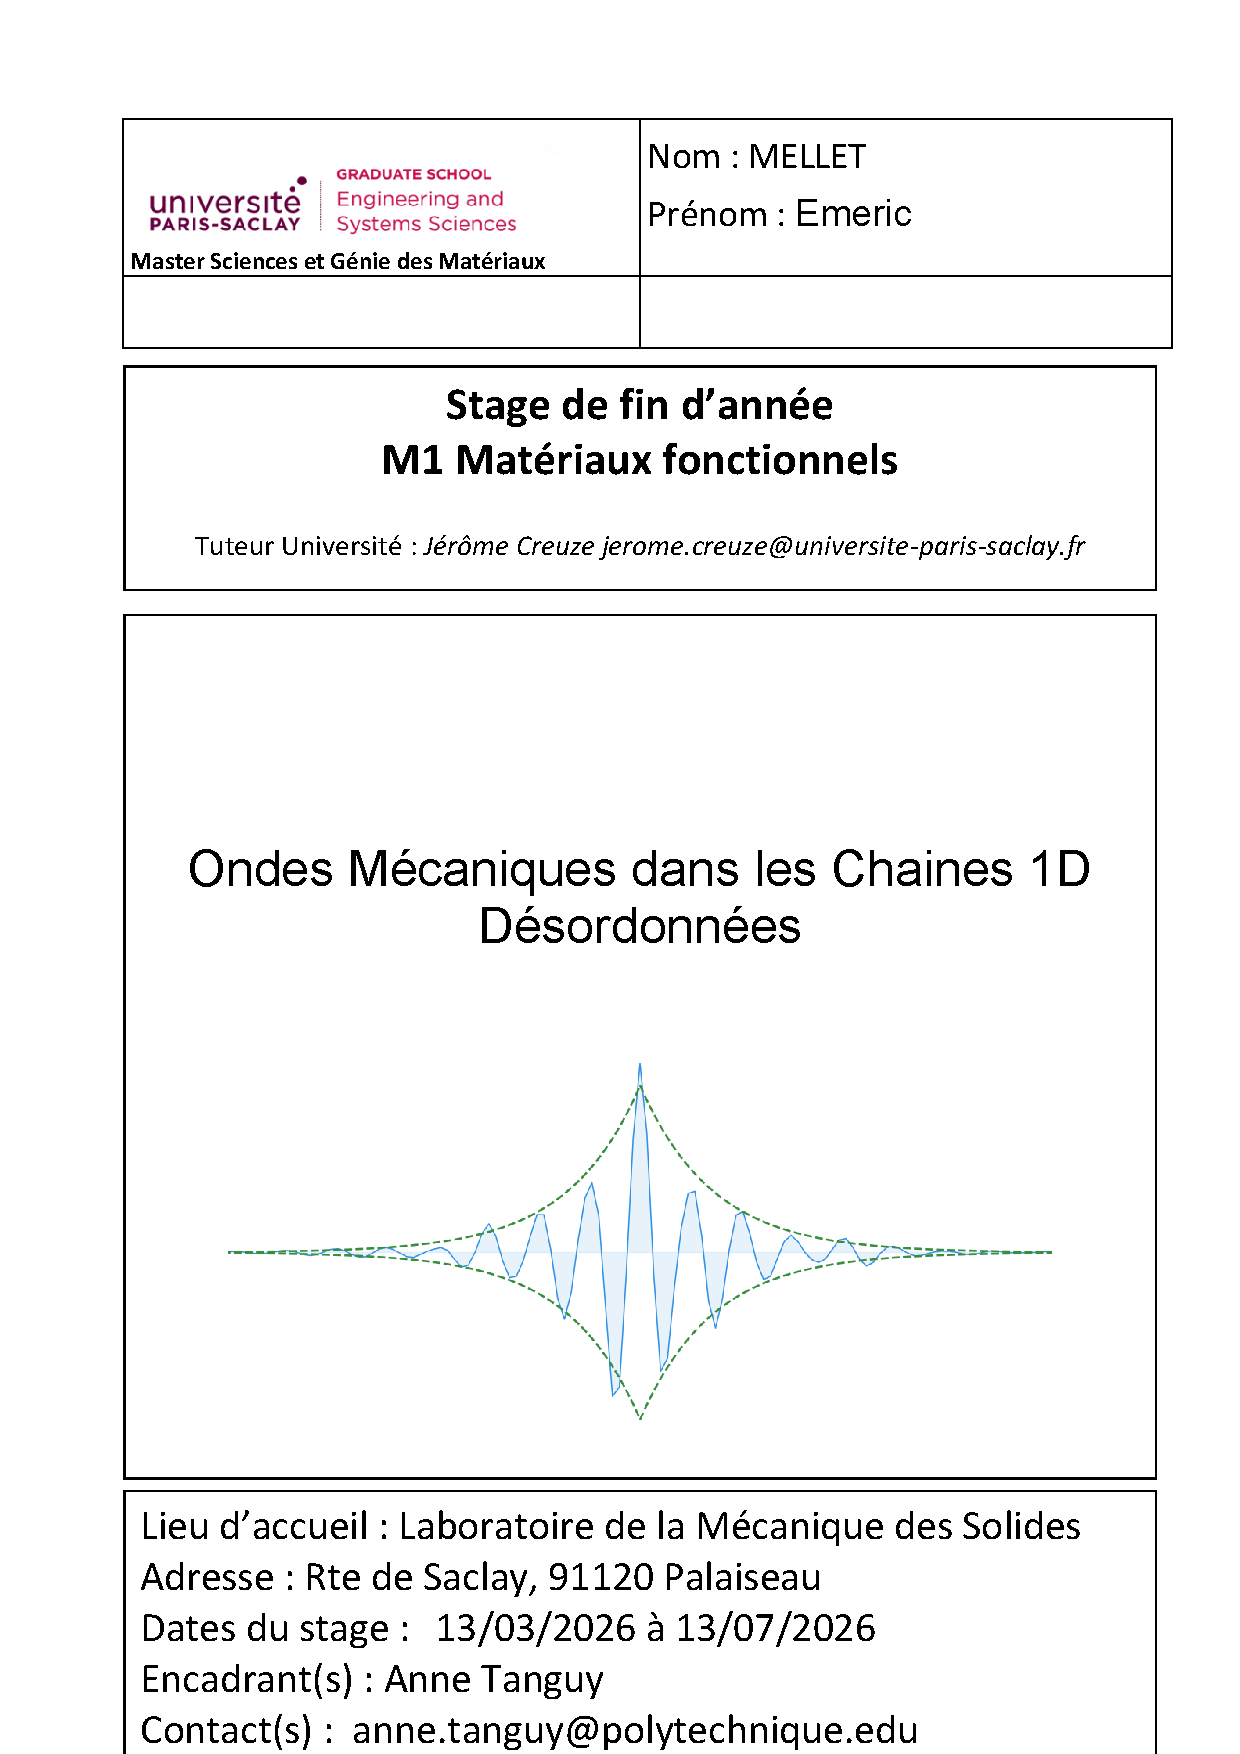
\includegraphics[width=\paperwidth,height=\paperheight,page=1]{template_ecampus.pdf}
        };
    \end{tikzpicture}
\end{titlepage}

\section*{Résumé / Abstract}
\begin{otherlanguage}{french}
\subsection*{Résumé}
Ce rapport présente une étude théorique et numérique de la propagation d'un paquet d'ondes au sein d'une chaîne unidimensionnelle constituée de masses et de ressorts, soumise aux effets du désordre structurel. L'analyse vise à quantifier l'impact des fluctuations stochastiques des masses ($m_i$) et des raideurs ($k_i$) sur le transport ondulatoire. Nous y caractérisons la transition entre le régime de propagation balistique et le régime de localisation forte, dans lequel l'énergie subit un confinement spatial exponentiel. Pour ce faire, les formalismes des matrices de transfert, de l'exposant de Lyapunov et du taux de participation sont comparés entre eux. Enfin, les résultats issus des simulations numériques de propagation de paquets d'onde sont confrontés aux prédictions analytiques de la théorie perturbative.

\vspace{0.5cm}
\noindent\textbf{Mots-clés :} Localisation, Transport ondulatoire, Chaîne harmonique 1D, Désordre structurel, Matrices de transfert, Exposant de Lyapunov.
\end{otherlanguage}

\vspace{1cm}

\begin{otherlanguage}{english}
\subsection*{Abstract}
This report presents a theoretical and numerical study of wave packet propagation within a one-dimensional mass-spring chain, subject to the effects of structural disorder. The analysis aims to quantify the impact of stochastic fluctuations in masses ($m_i$) and stiffnesses ($k_i$) on wave transport. We characterize the transition from the ballistic propagation regime to the strong localization regime, wherein energy undergoes an exponential spatial confinement. To achieve this, the formalisms of transfer matrices, Lyapunov exponent, and participation ratio are compared between themselves. Finally, the numerical results of wave packet propagation and attenuation are compared with analytical predictions derived from perturbative theory.

\vspace{0.5cm}
\noindent\textbf{Keywords:} Localization, Wave transport, 1D harmonic chain, Structural disorder, Transfer matrices, Lyapunov exponent.
\end{otherlanguage}

\newpage

% --- Remerciements ---
\section*{Remerciements}
\addcontentsline{toc}{section}{Remerciements}
Je tiens tout d'abord à exprimer ma profonde gratitude à mon encadrante de stage, Anne Tanguy. Au-delà de la confiance qu'elle m'a accordée dès le début, c'est sa rigueur scientifique et son esprit pédagogue qui ont été des moteurs de mon apprentissage. Ses conseils m'ont non seulement permis de progresser techniquement, mais m'ont surtout offert un regard plus affûté sur la démarche de recherche. Lors des points réguliers, elle a toujours su adapter ses explications à mon niveau, rendant des concepts plutôt complexes plus clairs.

Mes remerciements vont également au personnel du Laboratoire de Mécanique des Solides et des laboratoires voisins, qui m'ont accueilli et porté bienveillance. Je remercie particulièrement les chercheurs et doctorants pour leur accueil chaleureux et nos échanges, souvent informels. Ils m'ont permis de mieux appréhender le monde de la recherche et d'envisager plus sereinement mon avenir professionnel.

Enfin, je souhaite remercier les enseignants du Master 1 SGM de l'Université Paris-Saclay. Grâce aux enseignements dispensés, j'ai pu aborder les séminaires et les discussions techniques au sein du laboratoire avec plus d'aisance. Cette base théorique a été, pour moi, une véritable clé pour transformer mon stage en une expérience concrète et enrichissante.

\newpage

\tableofcontents

\newpage

% --- Introduction ---
\section*{Introduction} 
\addcontentsline{toc}{section}{Introduction}
\markboth{Introduction}{Introduction}

Ce stage a été effectué au sein du Laboratoire de Mécanique des Solides (LMS), hébergé à l'École Polytechnique. Ce laboratoire développe des recherches fondamentales et appliquées sur le comportement des matériaux et des structures, notamment sur les propriétés de couplage des matériaux amorphes et des structures non linéaires. Mon encadrante, Anne Tanguy, fait partie de ce laboratoire et travaille principalement sur les propriétés de transport ondulatoire dans des milieux désordonnés.

La mission scientifique de ce stage porte sur la caractérisation des phénomènes d'inhibition du transport vibratoire causés par des défauts structurels. L'objectif de mon travail est de quantifier le phénomène de localisation dans une chaîne 1D. Il s'agit de confronter les approches théoriques aux simulations numériques. Pour cela, des environnements de simulation en Python ont été développés afin d'implémenter des fluctuations stochastiques sur les masses et les raideurs. 

Ce rapport présente les méthodes employées et les résultats obtenus. Le premier chapitre présente l'état de l'art et rappelle les fondements théoriques de la dynamique des réseaux monoatomiques ordonnés avant de poser le formalisme de la localisation d'Anderson. Le deuxième chapitre est consacré à la modélisation de la chaîne harmonique stochastique, détaillant les méthodes de simulation temporelle (schéma de Leapfrog Verlet), d'analyse modale et de calcul de la longueur de localisation (méthode des matrices de transfert et Riccati). Le troisième chapitre expose les résultats numériques obtenus, comparant l'atténuation spatio-temporelle des paquets d'ondes aux mesures stationnaires. Le quatrième chapitre confronte ces résultats numériques aux prédictions analytiques de la théorie d'échelle (loi de Matsuda-Ishii). Enfin, nous discuterons de l'ouverture de ces travaux vers la physique des milieux amorphes et la relaxation thermique avant de conclure sur les perspectives de recherche, en particulier l'influence des non-linéarités sur le transport d'énergie.

\newpage

% --- État de l'Art ---
\section{État de l'Art : Dynamique des Chaînes 1D}

L'étude de la localisation des ondes dans les milieux désordonnés a été développée par Philip W. Anderson~\cite{anderson1958}. Il a démontré que l'introduction d'un désordre spatial aléatoire brise la symétrie de translation du milieu et peut entraîner la transition d'un régime conducteur vers une phase isolante où tout transport diffusif est inhibé. Cette notion, initialement formulée pour décrire la transition métal-isolant des électrons dans les solides désordonnés, s'est étendue à une grande variété de phénomènes physiques régis par des équations d'ondes classiques, notamment les ondes lumineuses, acoustiques et élastiques~\cite{skipetrov2010localisation, hu2008localization}. Les différents régimes de propagation, ainsi que l'évolution temporelle de la variance spatiale associée, sont illustrés schématiquement sur la Figure~\ref{fig:historical_context}.

\begin{figure}[ht!]
\centering
\includegraphics[width=1.0\textwidth]{01_historical_context.pdf}
\caption{\textbf{Régimes de transport ondulatoire dans les milieux 3D désordonnés.} Schéma des différents comportements de propagation d'une onde : (A) transport balistique dans un cristal parfait décrit par l'onde plane~\eqref{eq:bloch_wave}, (B) régime diffusif sous faible désordre, (C) localisation d'Anderson sous fort désordre caractérisée par la longueur de localisation~\eqref{eq:xi_lyapunov}, et (D) évolution de la variance spatiale associée $\sigma^2(t)$ pour ces trois régimes.}
\label{fig:historical_context}
\end{figure}

L'objectif de ce travail est d'étudier le cas unidimensionnel. Contrairement aux systèmes tridimensionnels (3D), qui présentent un seuil de mobilité, c'est à dire un seuil de fréquence au-dessus duquel les états se localisent, la théorie d'échelle de la localisation développée par \textcite{abrahams1979scaling} montre qu'en dimension $d=1$, tout désordre structurel entraîne la localisation exponentielle de tous les états propres. Cependant, la loi d'échelle de Matsuda-Ishii~\cite{matsuda1970localization} montre que la longueur de localisation $\xi$ diverge à basse fréquence dans la limite acoustique ($\xi \propto \omega^{-2}$), ce qui permet aux ondes de grande longueur d'onde de se propager sur de grandes distances avant d'être atténuées.

Pour estimer et quantifier la longueur de localisation, plusieurs approches théoriques complémentaires sont développées : l'approche perturbative de \textcite{matsuda1970localization} pour le régime acoustique basse fréquence, le formalisme exact de la matrice de transfert (TMM) développé par \textcite{schmidt1957disordered}, l'analyse de phase par la transformation de Riccati~\cite{halperin1965properties}, ainsi que les mesures globales basées sur le taux de participation modal (PR). Dans la limite du désordre faible, le développement perturbatif de Derrida et Gardner~\cite{derrida1984lyapounov} fournit également un formalisme précis. Ces différents modèles permettent de relier le désordre microscopique aux propriétés globales du champ d'ondes.

\FloatBarrier
\subsection{Réseau Ordonné et Relation de Dispersion}

\subsubsection{Chaîne Monoatomique Ordonnée}
Considérons une chaîne monoatomique idéale infinie constituée de masses identiques $m$ reliées par des ressorts de raideur identique $K$. Chaque masse (ou oscillateur) définit un \textit{site} du réseau, indexé par l'entier $n$. La distance d'équilibre entre deux sites adjacents est notée $a$. Notons $u_n(t)$ le déplacement longitudinal du site $n$ par rapport à sa position d'équilibre $x_n^0 = n a$. Dans l'approximation harmonique, la force de rappel exercée sur la masse au site $n$ dépend uniquement de ses plus proches voisins $n-1$ et $n+1$. L'équation du mouvement linéaire s'écrit alors :
\begin{equation}\label{eq:eom_chain}
    m \ddot{u}_n = K(u_{n+1} - u_n) - K(u_n - u_{n-1}) = K(u_{n+1} + u_{n-1} - 2u_n)
\end{equation}

Grâce à l'invariance par translation discrète du réseau, nous pouvons chercher des solutions sous la forme d'ondes planes de Bloch :
\begin{equation}\label{eq:bloch_wave}
    u_n(t) = U_0 e^{i(q n a - \omega t)}
\end{equation}
où $U_0$ désigne l'amplitude de l'onde, $q$ le vecteur d'onde (restreint à la première zone de Brillouin $q \in [-\pi/a, \, \pi/a]$) et $\omega$ la pulsation temporelle. En substituant l'expression de l'onde de Bloch~\eqref{eq:bloch_wave} dans l'équation du mouvement~\eqref{eq:eom_chain}, on obtient la relation suivante :
\begin{equation*}
    -m \omega^2 U_0 e^{i(q n a - \omega t)} = K U_0 e^{i(q n a - \omega t)} \left( e^{iqa} + e^{-iqa} - 2 \right)
\end{equation*}
En simplifiant par le facteur commun $U_0 e^{i(q n a - \omega t)}$, nous obtenons l'équation aux valeurs propres de dispersion :
\begin{equation*}
    -m \omega^2 = K \left( 2\cos(qa) - 2 \right) = -4K \sin^2\left(\frac{qa}{2}\right)
\end{equation*}
Ce qui conduit à la relation de dispersion de Brillouin~\cite{brillouin1953wave} :
\begin{equation}\label{eq:dispersion_mono}
    \omega(q) = 2\sqrt{\frac{K}{m}} \left| \sin\left(\frac{qa}{2}\right) \right| = \omega_{\max} \left| \sin\left(\frac{qa}{2}\right) \right|
\end{equation}
où $\omega_{\max} = 2\sqrt{K/m}$ est la pulsation de coupure supérieure du réseau ordonné. Au-delà de cette pulsation, le vecteur d'onde $q$ devient complexe, traduisant l'existence d'ondes évanescentes qui s'atténuent exponentiellement dans une chaîne parfaite.

La vitesse de groupe $v_g$ de l'onde est donnée par la dérivée de la relation de dispersion par rapport au vecteur d'onde :
\begin{equation*}
    v_g(q) = \frac{d\omega}{dq} = a\sqrt{\frac{K}{m}} \cos\left(\frac{qa}{2}\right) \mathrm{sgn}(q)
\end{equation*}
À basse fréquence ($q \to 0$), la relation de dispersion est linéaire et la vitesse de groupe est constante et égale à la vitesse du son macroscopique $c_0 = a\sqrt{K/m}$. Aux bords de la zone de Brillouin, la vitesse de groupe s'annule ($v_g = 0$), ce qui correspond à la formation d'une onde stationnaire.

La densité d'états vibrationnels $g(\omega)$ représente le nombre de modes de vibration par intervalle de fréquence unitaire. Pour un système 1D de taille $L = N a$, le nombre de modes dans la zone de Brillouin est conservé. En convertissant la somme discrète sur les modes en intégrale continue sur le vecteur d'onde, on obtient la densité d'états par site :
\begin{equation*}
    g(\omega) = \frac{a}{\pi} \frac{1}{\left| \frac{d\omega}{dq} \right|} = \frac{a}{\pi} \frac{1}{a\sqrt{\frac{K}{m}} \cos\left(\frac{qa}{2}\right)}
\end{equation*}
En exprimant le terme $\cos(qa/2)$ en fonction de $\omega$ via~\eqref{eq:dispersion_mono}, on obtient la densité d'états analytique :
\begin{equation}\label{eq:dos_mono}
    g(\omega) = \frac{2}{\pi} \frac{1}{\sqrt{\omega_{\max}^2 - \omega^2}}
\end{equation}
Cette densité d'états diverge à la coupure supérieure $\omega \to \omega_{\max}$ (voir Figure~\ref{fig:dispersion_monoatomic}). Cette divergence, caractéristique des systèmes unidimensionnels, est connue sous le nom de singularité de Van Hove.

\begin{figure}[ht!]
\centering
\includegraphics[width=1.0\textwidth]{02_dispersion.pdf}
\caption{\textbf{Relation de dispersion et densité d'états d'une chaîne monoatomique ordonnée.} Représentation graphique de la relation de dispersion $\omega(q)$ définie par~\eqref{eq:dispersion_mono} et de la densité d'états (DOS) $g(\omega)$ analytique donnée par~\eqref{eq:dos_mono}, montrant la singularité de Van Hove à la coupure supérieure.}
\label{fig:dispersion_monoatomic}
\end{figure}

% \FloatBarrier
\subsection{Désordre et Formalisme de Localisation}

Dans un solide réel, le réseau atomique présente des impuretés, des lacunes, des défauts cristallins ou des fluctuations de composition chimique. Ces imperfections se modélisent mathématiquement par l'introduction d'un désordre structurel stochastique sur les masses $m_n$ et/ou sur les raideurs des ressorts $K_n$, brisant l'invariance spatiale par translation. En conséquence, le théorème de Bloch~\eqref{eq:bloch_wave} n'est plus applicable. Les ondes de propagation subissent de multiples diffusions sur les fluctuations stochastiques du réseau.

\subsubsection{Longueur de Localisation et Exposant de Lyapunov}
La longueur de localisation d'Anderson $\xi(\omega)$ caractérise l'échelle spatiale typique de décroissance exponentielle du module du champ d'ondes vibrationnelles $|\psi_n| \sim e^{-n/\xi}$. Pour un réseau semi-infini, cette décroissance est quantifiée rigoureusement par l'exposant de Lyapunov $\gamma(\omega)$, défini comme le taux de croissance spatial asymptotique moyen du champ :
\begin{equation*}
    \gamma(\omega) = - \lim_{n \to \infty} \frac{1}{n} \left\langle \ln \left| \frac{u_n}{u_0} \right| \right\rangle
\end{equation*}
où les crochets $\langle \cdot \rangle$ représentent la moyenne d'ensemble sur les réalisations statistiques du désordre. La longueur de localisation physique $\xi(\omega)$ s'identifie à l'inverse de la partie réelle de l'exposant de Lyapunov :
\begin{equation}\label{eq:xi_lyapunov}
    \xi(\omega) = \frac{a}{\operatorname{Re}(\gamma(\omega))}
\end{equation}

Pour calculer $\gamma(\omega)$, la chaîne est discrétisée sous la forme d'un produit de matrices de transfert aléatoires $\mathbf{T}_i$. Le théorème mathématique de Furstenberg pour les produits de matrices de transfert aléatoires indépendantes et identiquement distribuées garantit que la norme du produit croît exponentiellement avec le nombre de matrices $N$ :
\begin{equation}\label{eq:furstenberg_limit}
    \lim_{N \to \infty} \frac{1}{N} \ln \left\| \prod_{i=1}^N \mathbf{T}_i \right\| = \gamma(\omega) > 0
\end{equation}
Ce théorème assure mathématiquement que la longueur de localisation $\xi(\omega)$ reste finie pour tout $\omega > 0$ en présence de désordre (voir le schéma du formalisme sur la Figure~\ref{fig:transfer_flowchart}).

\begin{figure}[ht!]
\centering
\includegraphics[width=0.9\textwidth]{06_transfer_flowchart.pdf}
\caption{\textbf{Formalisme des matrices de transfert et divergence spatiale.} Représentation du couplage des vecteurs d'état successifs par la relation~\eqref{eq:transfer_relation} sous l'effet du désordre local, illustrant comment le produit cumulé des matrices diverge exponentiellement conformément au théorème de Furstenberg défini par~\eqref{eq:furstenberg_limit}.}
\label{fig:transfer_flowchart}
\end{figure}

\subsubsection{Loi de Matsuda-Ishii et Limite Acoustique}
Dans la limite basse fréquence (régime acoustique, $\omega \to 0$), la longueur d'onde $\lambda = 2\pi/q$ devient très grande devant la distance interatomique $a$. L'onde élastique moyenne les fluctuations microscopiques du réseau, ce qui réduit l'efficacité de la diffusion. En développant l'exposant de Lyapunov au second ordre, \textcite{matsuda1970localization} ont établi la loi de comportement asymptotique pour la longueur de localisation :
\begin{equation}\label{eq:matsuda_law}
    \xi(\omega) \approx \frac{8 c_0^2}{\sigma_{\mathrm{eff}}^2 \omega^2} = \frac{8 K_0/m_0}{\sigma_{\mathrm{eff}}^2 \omega^2}
\end{equation}
où $c_0 = a\sqrt{K_0/m_0}$ est la vitesse du son du réseau ordonné de référence, et $\sigma_{\mathrm{eff}}^2$ la variance effective du désordre. La dépendance en $\omega^{-2}$ est identique pour le désordre de masse $m_n = m_0(1+\varepsilon X_n)$ et pour le désordre de raideur $K_n = K_0(1+\varepsilon Y_n)$ (où $X_n$ et $Y_n$ sont des variables aléatoires centrées de variance unitaire, et $\varepsilon$ l'amplitude du désordre). Cependant, la définition de la variance effective $\sigma_{\mathrm{eff}}^2$ dépend du type de désordre :
\begin{itemize}
    \item Pour le désordre de masse (diagonal), les fluctuations de masse $\epsilon_{n,m} = (m_n - m_0)/m_0$ agissent comme un potentiel stochastique, ce qui donne $\sigma_{\mathrm{eff}}^2 = \sigma_m^2 = \operatorname{Var}(\epsilon_{n,m}) = \varepsilon^2$.
    \item Pour le désordre de raideur (hors-diagonal), le désordre affecte les couplages. Comme montré dans la Section~\ref{subsubsec:riccati}, le développement perturbatif est réalisé sur les fluctuations de compliance $1/K_n$ par rapport à la moyenne harmonique de Reuss $\langle 1/K \rangle$ pour éviter un biais de premier ordre. La variance effective correspond à celle de la compliance relative : $\sigma_{\mathrm{eff}}^2 = \sigma_K^2 = \operatorname{Var}(1/K_n) / \langle 1/K_n \rangle^2 \approx \varepsilon^2$.
    \item Pour le désordre combiné (masses et raideurs), les deux contributions s'additionnent en limite acoustique : $\sigma_{\mathrm{eff}}^2 \approx \sigma_m^2 + \sigma_K^2$.
\end{itemize}

Cette loi de Matsuda-Ishii (loi en $\omega^{-2}$) indique que la longueur de localisation diverge lorsque la fréquence tend vers zéro. Les ondes acoustiques de très basse fréquence peuvent donc se propager sur des distances macroscopiques sans subir d'atténuation significative, assurant ainsi la transmission mécanique du son à longue distance dans les solides amorphes ou désordonnés. Cette divergence en $\omega^{-2}$ est spécifique à la dimension $d=1$ et diffère de la diffusion Rayleigh tridimensionnelle classique (qui prédit un libre parcours moyen $\ell \propto \omega^{-4}$). La confrontation de cette loi aux simulations exactes permet de tracer les limites d'admissibilité de la théorie perturbative.

% --- Modélisation ---
\section{Modélisation de la Chaîne Harmonique}

Pour simuler la dynamique vibrationnelle et caractériser la localisation des ondes, trois approches numériques complémentaires ont été développées en Python : l'intégration temporelle directe, la diagonalisation modale exacte, et le calcul stationnaire par matrices de transfert. Pour toutes ces simulations, nous choisissons de normaliser l'échelle d'espace en posant la distance intermasse $a = 1$, de sorte que l'unité de longueur correspond à la cellule élémentaire (le site du réseau). De même, nous fixons les paramètres physiques du réseau ordonné de référence à $m_0 = 1{,}0$ pour la masse et $K_0 = 1{,}0$ pour la raideur. Ce choix définit les unités de masse et de temps du système, fixant la pulsation maximale théorique du réseau ordonné à $\omega_{\max}^0 = 2\sqrt{K_0/m_0} = 2$. Dans ce système d'unités normalisé, le vecteur d'onde $q$ et le produit $qa$ sont numériquement identiques, ce qui rend le vecteur d'onde $q$ lui-même adimensionnel.


\FloatBarrier
\subsection{Simulation Temporelle et Schéma Symplectique}
Pour simuler la propagation transitoire d'ondes dans la chaîne, nous résolvons numériquement les équations différentielles couplées du mouvement. Le système d'équations pour les $N$ masses s'écrit sous forme matricielle :
\begin{equation*}
    \mathbf{M} \ddot{\mathbf{u}}(t) + \mathbf{G} \dot{\mathbf{u}}(t) + \mathbf{K} \mathbf{u}(t) = \mathbf{F}_{\text{ext}}(t)
\end{equation*}
où $\mathbf{u}(t)$ est le vecteur des déplacements, $\mathbf{M}$ la matrice diagonale des masses, $\mathbf{K}$ la matrice tridiagonale de raideur, $\mathbf{G}$ la matrice diagonale des coefficients d'amortissement aux bords, et $\mathbf{F}_{\text{ext}}(t)$ la force d'excitation externe. L'excitation temporelle modélisant le paquet d'ondes est appliquée sur le nœud central $n_0 = N/2$ sous la forme d'une impulsion gaussienne modulée :
\begin{equation}
    F_{\text{ext}, n}(t) = \delta_{n, n_0} F_0 \exp\left( -2 \sigma (t - t_0)^2 \right) \sin\left( \omega_{\text{ext}} (t - t_0) \right)
    \label{eq:f_ext_expression}
\end{equation}
où $\omega_{\text{ext}}$ désigne la pulsation de l'onde injectée et $\sigma$ le paramètre de sa largeur temporelle. Pour que le paquet d'ondes contienne $4$ oscillations (soit une durée caractéristique de $8\pi/\omega_{\text{ext}}$) et pour maintenir une largeur de bande fréquentielle relative $\Delta\omega/\omega_{\text{ext}}$ constante pour toutes les fréquences excitées, le paramètre $\sigma$ est défini par $\sigma = 1 / (4 \sigma_t^2)$ avec la constante de temps $\sigma_t = 8\pi / \omega_{\text{ext}}$, soit $\sigma = \omega_{\text{ext}}^2 / (256 \pi^2)$.

L'intégration temporelle est réalisée par l'algorithme symplectique de Leapfrog Verlet~\cite{hockney1970potential}. Contrairement aux intégrateurs classiques de type Runge-Kutta, les schémas symplectiques conservent la structure hamiltonienne et le volume de l'espace des phases du système. Cette propriété géométrique empêche toute dérive systématique de l'énergie mécanique sur de longues durées de simulation. Pour un pas de temps $\Delta t$, les variables de déplacement $u_j$ et de vitesse $v_j$ sont mises à jour selon le schéma à deux demi-pas :
\begin{align*}
    v_j\left(t + \frac{\Delta t}{2}\right) &= v_j(t) + \frac{\Delta t}{2} a_j(t) \\
    u_j(t + \Delta t) &= u_j(t) + \Delta t v_j\left(t + \frac{\Delta t}{2}\right) \\
    a_j(t + \Delta t) &= \frac{1}{m_j} \left[ F_j^{\text{élastique}}\big(\mathbf{u}(t + \Delta t)\big) - g_j v_j\left(t + \frac{\Delta t}{2}\right) + F_{\text{ext}, j}(t + \Delta t) \right] \\
    v_j(t + \Delta t) &= v_j\left(t + \frac{\Delta t}{2}\right) + \frac{\Delta t}{2} a_j(t + \Delta t)
\end{align*}

Pour garantir la stabilité numérique du schéma explicite, le pas de temps doit respecter la condition de Courant-Friedrichs-Lewy (CFL) :
\begin{equation*}
    \Delta t < \Delta t_{\text{crit}} = \frac{2}{\omega_{\max}} = \sqrt{\frac{m_0}{K_0}}
\end{equation*}
Si cette condition n'est pas remplie, les amplitudes des modes de haute fréquence croissent de façon exponentielle, provoquant une divergence numérique.

\begin{figure}[ht!]
\centering
\includegraphics[width=1.0\textwidth]{04_disordered_chain_schematic.pdf}
\caption{\textbf{Configuration spatiale de la chaîne d'oscillateurs modélisée.} Schéma du réseau numérique unidimensionnel mettant en évidence le nœud central d'excitation piloté par la force temporelle~\eqref{eq:f_ext_expression}, la région désordonnée et les couches absorbantes (ABC) caractérisées par le profil quadratique d'amortissement~\eqref{eq:absorbing_profile}.}
\label{fig:disordered_chain_schematic}
\end{figure}

Pour modéliser un réseau infini sur un domaine numérique fini de taille $N$, des conditions aux limites absorbantes (\textit{Absorbing Boundary Conditions}, ABC) sont implémentées aux extrémités gauche et droite du réseau. Les couches absorbantes de largeur $L_{\text{ABC}}$ introduisent un amortissement visqueux local $g_j$. Afin d'éviter les réflexions d'ondes indésirables à l'interface entre la zone physique centrale et la zone absorbante, le coefficient d'amortissement $g_j$ augmente de manière continue et progressive selon un profil quadratique (voir Figure~\ref{fig:disordered_chain_schematic}) :

\begin{equation}\label{eq:absorbing_profile}
    g_j = g_{\max} \left( \frac{x_j - x_{\text{abc}}}{L_{\text{abc}}} \right)^2
\end{equation}

En régime stationnaire harmonique, des conditions de radiation exactes (RBC) utilisant des impédances complexes $z(\omega) = e^{iq(\omega)a}$ sont appliquées aux bords pour éliminer totalement les réflexions.

\FloatBarrier
\subsection{Analyse Modale et Symétrisation du Problème}
L'analyse modale cherche les modes vibrationnels stationnaires de la chaîne libre de vibrations en posant $\mathbf{u}(t) = \tilde{\mathbf{u}} e^{i\omega t}$. Cela conduit à un problème aux valeurs propres généralisé :

\begin{equation}\label{eq:gen_eig}
    \mathbf{K} \tilde{\mathbf{u}} = \omega^2 \mathbf{M} \tilde{\mathbf{u}}
\end{equation}

Dans un système désordonné, la matrice des masses $\mathbf{M}$ est diagonale et la matrice de raideur $\mathbf{K}$ est tridiagonale, mais toutes deux sont non uniformes. Pour résoudre ce problème de manière stable et performante à l'aide de solveurs standards, il est nécessaire de ramener ce problème aux valeurs propres généralisé à un problème standard symétrique. La matrice des masses $\mathbf{M}$ étant diagonale et strictement positive, sa racine carrée $\mathbf{M}^{1/2}$ et son inverse $\mathbf{M}^{-1/2}$ sont bien définies et diagonales. On pose alors le changement de variable (déplacement pondéré par la masse) :
\begin{equation*}
    \mathbf{v} = \mathbf{M}^{1/2} \tilde{\mathbf{u}} \quad \Longleftrightarrow \quad \tilde{\mathbf{u}} = \mathbf{M}^{-1/2} \mathbf{v}
\end{equation*}
soit en composantes $v_n = \sqrt{m_n} \tilde{u}_n$. En injectant cette expression de $\tilde{\mathbf{u}}$ dans l'équation~\eqref{eq:gen_eig}, on obtient :
\begin{equation*}
    \mathbf{K} \mathbf{M}^{-1/2} \mathbf{v} = \omega^2 \mathbf{M} \mathbf{M}^{-1/2} \mathbf{v}
\end{equation*}
En multipliant cette relation à gauche par $\mathbf{M}^{-1/2}$, il vient :
\begin{equation*}
    \left(\mathbf{M}^{-1/2} \mathbf{K} \mathbf{M}^{-1/2}\right) \mathbf{v} = \omega^2 \left(\mathbf{M}^{-1/2} \mathbf{M} \mathbf{M}^{-1/2}\right) \mathbf{v}
\end{equation*}
Puisque $\mathbf{M}^{-1/2} \mathbf{M} \mathbf{M}^{-1/2} = \mathbf{I}$ (la matrice identité), on obtient le problème aux valeurs propres standard symétrique :
\begin{equation}\label{eq:sym_eig}
    \mathbf{D} \mathbf{v} = \omega^2 \mathbf{v}
\end{equation}
où la matrice dynamique symétrisée $\mathbf{D}$ est définie par :
\begin{equation*}
    \mathbf{D} = \mathbf{M}^{-1/2} \mathbf{K} \mathbf{M}^{-1/2}
\end{equation*}
Les éléments non nuls de cette matrice tridiagonale symétrique réelle sont :
\begin{align*}
    D_{n,n} &= \frac{K_n + K_{n-1}}{m_n} \\
    D_{n, n+1} = D_{n+1, n} &= -\frac{K_n}{\sqrt{m_n m_{n+1}}}
\end{align*}
La diagonalisation numérique de $\mathbf{D}$ fournit des valeurs propres $\omega_i^2$ réelles positives et un ensemble de vecteurs propres orthonormaux $\mathbf{v}_i$, à partir desquels on reconstruit les modes physiques $\tilde{\mathbf{u}}_i = \mathbf{M}^{-1/2} \mathbf{v}_i$.

L'introduction de désordre sur la diagonale (masses) ou hors-diagonale (raideurs) modifie la propagation de l'onde. Le désordre atténue la singularité de Van Hove et élargit le spectre au-delà de la limite théorique $\omega_{\max}^0 = 2$ (voir Figure~\ref{fig:spectral_asymmetry}). Les fluctuations stochastiques permettent l'apparition locale de configurations de masse ou de raideur qui agissent comme des résonateurs isolés à haute fréquence. Ces états localisés forment des "queues de Lifshitz" dans la densité d'états (voir Figure~\ref{fig:spectral_asymmetry}), caractéristique des milieux désordonnés amorphes.

\begin{figure}[ht!]
\centering
\includegraphics[width=1.0\textwidth]{05_spectral_asymmetry.pdf}
\caption{\textbf{Érosion de la singularité de Van Hove et queues de Lifshitz.} (a) Densité d'états (DOS) perturbée pour un désordre stochastique de masse ou de raideur ($\sigma_\varepsilon = 0{,}9$) comparée à la solution analytique de la chaîne ordonnée~\eqref{eq:dos_mono}. (b) Zoom en échelle logarithmique sur les queues de Lifshitz formées par des modes propres localisés au-delà de la coupure théorique $\omega_{\max}^0 = 2$.}
\label{fig:spectral_asymmetry}
\end{figure}

\FloatBarrier
\subsection{Indicateurs Spatiaux et Formalisme Matriciel}

\subsubsection{Taux de Participation}
Pour quantifier l'extension spatiale d'un mode propre $\psi$, nous utilisons le taux de participation (\textit{Participation Ratio}, $PR_{\text{ratio}}$), défini par :
\begin{equation}\label{eq:pr_definition}
    PR_{\text{ratio}}(\psi) = \frac{1}{N} \frac{\left( \sum_{n=1}^N |\psi_n|^2 \right)^2}{\sum_{n=1}^N |\psi_n|^4}
\end{equation}
Ce ratio, compris entre $1/N$ (localisation maximale sur un seul site) et $1$ (délocalisation complète), estime la proportion de sites du réseau actifs dans le mode de vibration. 

Pour comparer directement cet indicateur à la longueur de localisation $\xi$ (exprimée en nombre de sites), nous utilisons le nombre de participation $PR = N \cdot PR_{\text{ratio}}$. Pour un mode totalement délocalisé (onde plane uniforme $|\psi_n| = 1/\sqrt{N}$), on a $PR = N$, tandis que pour un mode localisé sur un site unique, $PR = 1$. Bien que le nombre de participation et la longueur de localisation décrivent des concepts physiques différents (l'occupation globale contre le taux de décroissance exponentielle), ils prennent des valeurs proches sur une grande partie de la chaîne.

Ce nombre de participation est sujet aux effets de taille finie : sa valeur maximale est bornée par la taille $N$ du réseau. Lorsque la longueur de localisation $\xi$ dépasse la taille du réseau ($\xi \gg N$), le nombre $PR$ sature à $N$, ce qui masque la longueur de localisation réelle. Pour s'affranchir de cette saturation, il faudrait augmenter la taille $N$ du système ; or, la diagonalisation numérique complète requise par l'analyse modale devient prohibitivement coûteuse en temps de calcul et en mémoire (de complexité $\mathcal{O}(N^3)$) pour de grands réseaux.

Afin de contourner ces limitations physiques et computationnelles, et d'évaluer précisément la longueur de localisation $\xi$ dans la limite thermodynamique ($N \to \infty$) — notamment pour un désordre très faible où $\xi$ est extrêmement grand —, il convient d'abandonner l'analyse modale statique au profit d'une méthode de propagation pas à pas : le formalisme de la matrice de transfert.


\subsubsection{Matrice de Transfert et Riccati}\label{subsubsec:riccati}

La methode de Riccati permet de calculer l'exposant de Lyapunov sans calculer les matrices de transfert. On commence avec l'equation du mouvement sur le site $n$ :

\begin{equation*}
    -m_n \omega^2 u_n = K_n(u_{n+1} - u_n) - K_{n-1}(u_n - u_{n-1})
\end{equation*}

Cette relation de récurrence du second ordre peut être mise sous la forme matricielle suivante en reliant les déplacements de deux sites successifs :

\begin{equation}\label{eq:transfer_relation}
    \begin{pmatrix} u_{n+1} \\ u_n \end{pmatrix} = \mathbf{T}_n(\omega) \begin{pmatrix} u_n \\ u_{n-1} \end{pmatrix}
\end{equation}

où la matrice de transfert $\mathbf{T}_n(\omega)$ est définie par :

\begin{equation}\label{eq:transfer_matrix_def}
    \mathbf{T}_n(\omega) = \begin{pmatrix} \frac{K_n + K_{n-1} - m_n \omega^2}{K_n} & -\frac{K_{n-1}}{K_n} \\ 1 & 0 \end{pmatrix}
\end{equation}

La propagation de l'onde à travers tout le réseau est alors représentée par le produit des matrices de transfert : $\mathbf{M}_N = \prod_{n=1}^N \mathbf{T}_n$.

\begin{figure}[ht!]
\centering
\includegraphics[width=1.0\textwidth]{07_eigenmodes_waterfall.pdf}
\caption{Profils spatiaux de modes propres sélectionnés à travers le spectre pour une chaîne désordonnée ($N=100$, $\sigma_\epsilon=0{,}9$). Les modes de basse fréquence sont étendus sur tout le système, tandis que les modes de haute fréquence se localisent sur un petit nombre de sites.}
\label{fig:eigenmodes_waterfall}
\end{figure}

Cependant, multiplier numériquement un grand nombre de matrices de transfert présente des instabilités importantes : les amplitudes croissent ou décroissent exponentiellement, provoquant rapidement des dépassements de capacité numérique (\textit{overflow} ou \textit{underflow}). Pour contourner cette difficulté, on réalise une transformation de Riccati en introduisant la variable de rapport d'amplitude :

\begin{equation*}
    R_n = \frac{u_{n+1}}{u_n}
\end{equation*}

En substituant $R_n$ dans l'équation de récurrence, on obtient une équation de Riccati non linéaire du premier ordre, qui reste exacte :

\begin{equation}\label{eq:riccati_rec}
    R_n = \frac{K_n + K_{n-1} - m_n\omega^2}{K_n} - \frac{K_{n-1}}{K_n R_{n-1}}
\end{equation}

Cette formulation scalaire~\eqref{eq:riccati_rec} est numériquement stable et permet de calculer directement l'exposant de Lyapunov exact $\gamma$ par une simple moyenne logarithmique :

\begin{equation*}
    \gamma(\omega) = \frac{1}{N} \sum_{n=1}^N \ln |R_n|
\end{equation*}

Afin d'évaluer la longueur de localisation, deux implémentations numériques de cette approche seront systématiquement comparées (notamment sur la Figure~\ref{fig:attenuation_methods}). En se restreignant à un désordre purement diagonal de masse ($K_n = K = 1, m_n = 1+\varepsilon_n$), la méthode dite <<~TMM~>> exploitera la forme exacte de la récurrence :
\begin{equation}\label{eq:tmm_computation}
    R_{n+1} = (2 - m_n\omega^2) - \frac{1}{R_n} \quad \text{avec} \quad \gamma_{\text{TMM}} = \frac{1}{N}\sum_{n=1}^N \ln|R_n|
\end{equation}
La méthode dite <<~Riccati~>> exploitera quant à elle le formalisme des phases stochastiques linéarisé (approche de Derrida-Gardner détaillée dans l'Annexe~\ref{annexe:derrida-derivation}). L'incrément de phase complexe $\eta_n$ y est mis à jour itérativement selon le développement au second ordre :
\begin{equation*}
    \eta_{n+1} = A_n(qa) + \frac{B_n(qa)}{|B_n(qa)|} \eta_n
\end{equation*}
où $a$ désigne la distance intermasse et $q$ le vecteur d'onde, le produit $qa$ représentant la phase adimensionnelle. Dans nos simulations numériques, l'échelle d'espace est normalisée en fixant $a = 1$, ce qui exprime toutes les longueurs (dont la longueur de localisation) en nombre de sites du réseau. Les coefficients de dérive et de diffusion ($A_n$ et $B_n$ respectivement) dépendent de cette phase et de la perturbation locale $\varepsilon_n$ :
\begin{equation*}
    f(q) = 2 e^{-iqa}(1 - \cos qa), \quad A_n(qa) = -f(q)\varepsilon_n - \frac{1}{2}f(q)^2\varepsilon_n^2, \quad B_n(qa) = e^{-2iqa} + f(q)\varepsilon_n
\end{equation*}

Afin d'optimiser l'évaluation numérique, cette relation de récurrence peut être déroulée analytiquement. En notant $B_k(qa)$ le coefficient de propagation (éventuellement normalisé en module), la phase accumulée s'exprime globalement sous la forme exacte employée dans nos algorithmes :
\begin{align}\label{eq:riccati_phase_global}
    \eta_n &= \left( \prod_{k=0}^{n-1} B_k(qa) \right) \eta_0 + \sum_{j=0}^{n-1} A_j(qa) \left( \prod_{k=j+1}^{n-1} B_k(qa) \right) \nonumber \\
    &= \left[ \eta_0 + \sum_{j=0}^{n-1} \frac{A_j(qa)}{\prod_{k=0}^{j} B_k(qa)} \right] \times \prod_{k=0}^{n-1} B_k(qa)
\end{align}
L'exposant de Lyapunov en est déduit par la dérive moyenne de la partie réelle : $\gamma_{\text{Ric}} = \frac{1}{N} \sum_{n=1}^N \Re(\eta_n)$.

Les détails formels des développements et des dérivations de ces formalismes de Riccati sont présentés dans l'Annexe~\ref{annexe:computational_logic} et l'Annexe~\ref{annexe:lyapunov-derivation}. C'est également à partir de cette formulation exacte de Riccati que sont construits les développements analytiques perturbatifs permettant d'extraire la loi limite de Matsuda-Ishii en désordre faible.

Cette reformulation recentrée n'altère pas le système physique, mais prévient l'accumulation d'un biais systématique de premier ordre lors de la propagation numérique. Le formalisme stochastique de Riccati (et le développement de Derrida-Gardner) postule des fluctuations de moyenne nulle ($\langle \varepsilon_n \rangle = 0$). Or, pour un désordre de raideur, la variable physique propagée est la compliance $1/K_n$. Du fait de la non-linéarité de l'inversion, un désordre symétrique sur $K_n$ génère des fluctuations de compliance non centrées ($\langle 1/K_n - 1 \rangle \neq 0$). Sans correction, ce biais (dérive stochastique artificielle) s'accumule exponentiellement sur de grands réseaux, faussant la longueur de localisation calculée. Le recentrage est obtenu en définissant le milieu de référence par la compliance moyenne $\langle 1/K \rangle$ (moyenne harmonique de Reuss). La variable de désordre recentrée s'écrit alors $\varepsilon_n = \frac{1/K_n - \langle 1/K \rangle}{\langle 1/K \rangle}$, garantissant $\langle \varepsilon_n \rangle = 0$ et la consistance du formalisme avec la loi de Matsuda-Ishii.

% --- Résultats ---
\section{Résultats et Simulations}

Les simulations numériques menées sur des chaînes de grande taille permettent d'observer directement les manifestations physiques de la localisation, autant dans le domaine spectral que dans le domaine temporel.

\FloatBarrier
\subsection{Modes propres de la matrice dynamique en présence de désordre}

\subsubsection{Taux de participation et densité d'états}
L'analyse modale statistique du système de taille $N=6000$ met en évidence la signature spectrale de la localisation. La Figure~\ref{fig:participation_ratio} illustre l'évolution conjointe de la densité d'états et du taux de participation moyen pour trois intensités de désordre de raideur.

\begin{figure}[ht!]
\centering
\includegraphics[width=1.0\textwidth]{10_participation_ratio.pdf}
\caption{\textbf{Densité d'états et taux de participation sous désordre de raideur.} Distribution spectrale de la densité d'états (DOS) et du taux de participation moyen $PR(\psi)$ défini par~\eqref{eq:pr_definition} en fonction de la pulsation $\omega$ pour trois amplitudes de désordre de raideur ($\sigma_\varepsilon \in \{0{,}1;\, 0{,}7;\, 1{,}4\}$) sur un réseau de taille $N = 6000$.}
\label{fig:participation_ratio}
\end{figure}

Pour un désordre faible, la densité d'états reste proche de la courbe théorique du réseau ordonné. Elle présente notamment une divergence à la fréquence de coupure. Le taux de participation associé à ces modes est élevé, ce qui indique une délocalisation des modes sur l'ensemble de la chaîne, à l'exception de la région proche de la coupure.

Lorsque le désordre augmente, le spectre de la densité d'états s'élargit et le pic de la coupure diminue. Pour un désordre fort, la distribution s'étend vers les hautes fréquences. Le taux de participation associé à ces modes de haute fréquence diminue, ce qui montre la localisation des modes. À l'inverse, dans la limite basse fréquence, le taux de participation reste proche de $N$.

\FloatBarrier

\FloatBarrier
\subsubsection{Élargissement Spectral et Rupture de la Périodicité de Bloch}
Dans un réseau ordonné, les modes vibrationnels sont des ondes planes de Bloch caractérisées par un vecteur d'onde $q_0$ (le spectre de Fourier spatial est un pic de Dirac $\delta(q - q_0)$). L'introduction du désordre élargit le spectre de Fourier.

La Figure~\ref{fig:spectral_broadening} présente le spectre de Fourier spatial (densité spectrale en vecteur d'onde $q$) d'un paquet d'ondes excité à une fréquence $\omega$ dans une chaîne désordonnée. En raison de la localisation d'Anderson, l'enveloppe spatiale du mode décroît exponentiellement en $e^{-|x|/\xi}$. Mathématiquement, la transformée de Fourier spatiale d'une décroissance exponentielle symétrique est égale à un profil lorentzien (profil de Cauchy) centré sur le vecteur d'onde moyen $q_0$ :
\begin{equation}\label{eq:lorentzian_profile}
    I(q) \propto \frac{\Delta q}{\pi \left[ (q - q_0)^2 + (\Delta q)^2 \right]}
\end{equation}
La largeur à mi-hauteur $\Delta q$ de ce profil lorentzien est directement reliée à la longueur de localisation spatiale par la relation d'incertitude :
\begin{equation}\label{eq:uncertainty_relation}
    \Delta q = \frac{1}{\xi}
\end{equation}

Comme illustré sur la Figure~\ref{fig:spectral_broadening}, l'augmentation du désordre élargit le spectre. Le vecteur d'onde $q$ n'est plus conservé, la phase de l'onde étant modifiée sur une distance égale à la longueur de localisation $\xi$. Ce comportement est similaire à celui observé par diffusion inélastique de neutrons ou de rayons X dans les verres et les solides amorphes.


\begin{figure}[ht!]
\centering
\includegraphics[width=1.0\textwidth]{11_spectral_broadening.pdf}
\caption{\textbf{Élargissement de la densité spectrale spatiale sous l'effet du désordre.} Spectres de Fourier spatiaux du déplacement d'une onde comparés au profil lorentzien théorique~\eqref{eq:lorentzian_profile}. L'accroissement du désordre élargit la largeur à mi-hauteur $\Delta q$, reliée à la longueur de localisation $\xi$ par la relation d'incertitude~\eqref{eq:uncertainty_relation}, traduisant la perte de périodicité de Bloch.}
\label{fig:spectral_broadening}
\end{figure}

\FloatBarrier
\subsection{Approche analytique perturbative}

\subsubsection{Validation de la loi de Matsuda Ishii}
Dans la limite macroscopique basse fréquence ($\omega \to 0$), la longueur de localisation $\xi(\omega)$ suit la loi perturbative de Matsuda-Ishii~\eqref{eq:matsuda_law}. La Figure~\ref{fig:matsuda_ishii_scaling} présente la longueur de localisation extraite par la méthode de la matrice de transfert (TMM) pour différentes intensités de désordre de raideur ($\varepsilon \in \{0{,}1, \, 0{,}3, \, 1{,}5\}$) en fonction de la fréquence $\omega$.

\begin{figure}[ht!]
\centering
\includegraphics[width=1.0\textwidth]{12_matsuda_ishii.pdf}
\caption{\textbf{Validation de la loi limite de Matsuda-Ishii.} Confrontation de la longueur de localisation $\xi(\omega)$ mesurée par la méthode des matrices de transfert (TMM) avec la loi analytique basse fréquence~\eqref{eq:matsuda_law} pour trois amplitudes de désordre de raideur ($\varepsilon \in \{0{,}1;\, 0{,}3;\, 1{,}5\}$), mettant en évidence l'admissibilité du développement perturbatif.}
\label{fig:matsuda_ishii_scaling}
\end{figure}

Pour de faibles amplitudes de désordre ($\varepsilon = 0{,}1$ et $\varepsilon = 0{,}3$), l'accord entre le calcul exact TMM et la loi analytique en $\omega^{-2}$ est vérifié pour $\omega \in [0{,}1, \, 1{,}2]$. Cela valide l'approximation du développement perturbatif au second ordre, où l'atténuation résulte de la somme des fluctuations locales indépendantes.

Cependant, pour un fort désordre ($\varepsilon = 1{,}5$), on observe un écart entre la théorie et la simulation, en particulier aux fréquences intermédiaires et élevées. Le développement perturbatif au second ordre sous-estime l'atténuation du système. À fort désordre, les termes d'ordre supérieur et la diffusion multiple ne sont plus négligeables, réduisant la longueur de localisation en deçà de la valeur prédite par la théorie de Matsuda-Ishii. De plus, à l'approche de la fréquence de coupure $\omega \to \omega_{\max}^0 = 2$, la longueur de localisation diminue vers des valeurs de l'ordre de quelques sites, en raison de la transition vers le régime de queues de Lifshitz.

Pour quantifier ces écarts, des régressions linéaires sont effectuées dans le régime basse fréquence ($\omega \in [0{,}4, \, 1{,}2]$). Pour compenser les effets de bord de bande, on introduit la longueur de localisation compensée :
\begin{equation}
    \xi_{\mathrm{comp}}(\omega) = \frac{\xi(\omega)}{1 - \omega^2 / 4}
\end{equation}
La relation d'ajustement linéaire s'écrit alors en échelle logarithmique :
\begin{equation}
    \ln\big(\xi_{\mathrm{comp}}(\omega)\big) = -\alpha \ln(\omega) + \ln\left(\frac{8}{\sigma_{\mathrm{eff}}^2}\right)
\end{equation}
où la pente de la droite correspond à $-\alpha$, et l'ordonnée à l'origine $C$ permet d'extraire la force de désordre effective $\sigma_{\mathrm{eff}}^2 = 8 / \exp(C)$. 
La Figure~\ref{fig:scaling_fits_illustration} montre les courbes d'ajustement de la longueur d'atténuation $\xi(\omega)$ pour les désordres de masse, de raideur et combiné. Les exposants de scaling $\alpha$ extraits et les forces de désordre effectives $\sigma_{\mathrm{eff}}^2$ correspondantes sont confrontés aux prédictions théoriques sur la Figure~\ref{fig:parameters_comparison}.

\begin{figure}[ht!]
\centering
\includegraphics[width=1.0\textwidth]{14_scaling_fits_illustration.pdf}
\caption{\textbf{Régression linéaire et exposant de scaling de la longueur de localisation.} Ajustement linéaire de $\ln\xi_{\mathrm{comp}}$ en fonction de $\ln\omega$ dans le domaine $\omega \in [0{,}4;\, 1{,}2]$ pour (a) le désordre de masses, (b) le désordre de raideurs, et (c) le désordre combiné, visant à valider l'exposant $\alpha = 2$ de la loi asymptotique~\eqref{eq:matsuda_law}.}
\label{fig:scaling_fits_illustration}
\end{figure}

\begin{figure}[ht!]
\centering
\includegraphics[width=1.0\textwidth]{15_parameters_comparison.pdf}
\caption{\textbf{Comparaison des paramètres de scaling ajustés.} Paramètres de scaling extraits par régression linéaire pour les différents modèles numériques comparés aux prédictions théoriques de la relation~\eqref{eq:matsuda_law}. (a) Exposant de scaling $\alpha$, théoriquement égal à $2$. (b) Variance effective $\sigma_{\mathrm{eff}}^2$ comparée aux valeurs statistiques.}
\label{fig:parameters_comparison}
\end{figure}

Les résultats d'ajustement présentés sur la Figure~\ref{fig:parameters_comparison}(a) montrent que l'exposant de scaling $\alpha$ est proche de sa valeur théorique $\alpha = 2$ pour la méthode des matrices de transfert (TMM) et les taux de participation (PR). On observe cependant que la méthode de \og Riccati Numérique \fg{} s'en écarte significativement, s'élevant vers des valeurs de $\alpha \approx 2{,}5$ à $3$. Ce comportement singulier met en évidence la sensibilité de l'algorithme de Riccati dans le régime de très basse fréquence, où les fluctuations de phase cumulées lors de l'intégration le long de la chaîne perturbent l'extraction de la pente asymptotique.

Pourtant, comme l'illustre la Figure~\ref{fig:parameters_comparison}(b), la force du désordre effective $\sigma_{\mathrm{eff}}^2$ extraite par Riccati reste très bien alignée avec les autres méthodes et avec les prédictions théoriques. Contrairement aux versions antérieures, les corrections mathématiques apportées au formalisme permettent désormais d'estimer correctement l'intensité du désordre ($\sigma_{\mathrm{eff}}^2 \approx 0{,}02$ pour le désordre pur et $\approx 0{,}04$ pour le cas combiné), affranchissant cette mesure de l'erreur systématique observée sur l'exposant $\alpha$.

Les approches TMM et PR confirment également cette concordance. Il est crucial de rappeler que pour le désordre de raideur, l'accord avec la loi de Matsuda-Ishii n'est obtenu que si l'on centre rigoureusement la compliance (milieu effectif de Reuss). Sous cette condition physique, la force du désordre effective $\sigma_{\mathrm{eff}}^2$ issue de TMM concorde parfaitement avec la variance statistique théorique des fluctuations microscopiques introduites dans le système. Dans le cas du désordre combiné, on retrouve l'additivité attendue en limite acoustique ($\sigma_{\mathrm{eff, comb}}^2 \approx \sigma_m^2 + \sigma_K^2$). De plus, la normalisation $\xi_{PR} = PR$ permet d'obtenir pour le taux de participation des variances effectives très proches de celles issues de TMM, confirmant la pertinence de cet indicateur modal dans le régime d'échelle intermédiaire.

\FloatBarrier

\FloatBarrier
\subsubsection{Longueurs de localisation}

La Figure~\ref{fig:attenuation_methods} compare la longueur de localisation $\xi(\omega)$ obtenue par les cinq méthodes numériques et analytiques. L'accord sur la plage de pulsations $\omega \in [0{,}8,\,1{,}8]$ valide la cohérence de ces différentes approches.

\begin{figure}[p]
\centering
\includegraphics[width=1.0\textwidth,height=0.8\textheight,keepaspectratio]{13_attenuation_methods_comparison.pdf}
\caption{\textbf{Confrontation des méthodes d'extraction de la longueur de localisation.} Comparaison de la longueur d'atténuation $\xi(\omega)$ obtenue par matrices de transfert (TMM)~\eqref{eq:tmm_computation}, récurrence scalaire de Riccati stochastique~\eqref{eq:riccati_phase_global}, loi asymptotique de Matsuda-Ishii~\eqref{eq:matsuda_law}, taux de participation des modes propres~\eqref{eq:pr_definition}, et enveloppe exponentielle du paquet d'ondes~\eqref{eq:exponential_decay_wp}.}
\label{fig:attenuation_methods}
\end{figure}

À basse fréquence ($\omega \to 0$), $\xi_{PR}$ sature à $N/3 \approx 2000$ sites alors que $\xi$ diverge. Cette saturation se produit lorsque $\xi > N$ : le mode propre s'étend sur la totalité de la chaîne et son taux de participation est borné par $N$. La méthode exacte TMM, formulée en régime semi-infini ouvert, ne présente pas cette limitation et reproduit fidèlement la divergence en $\omega^{-2}$ de la loi de Matsuda-Ishii~\eqref{eq:matsuda_law}. Bien que la méthode de Riccati Numérique diverge également, son instabilité itérative aux basses fréquences l'empêche de capturer correctement cet exposant asymptotique.

La confrontation confirme par ailleurs l'additivité des désordres de masse et de raideur à basse fréquence : $\sigma_{\mathrm{eff}}^2 = \sigma_m^2 + \sigma_K^2$, en accord avec la loi~\eqref{eq:matsuda_law}. À haute fréquence, le désordre de raideur domine, induisant une chute plus prononcée de $\xi$ à l'approche de la coupure $\omega_{\max}^0$.

% --- Discussion ---

\FloatBarrier
\subsection{Analyse spatio-temporelle du transport ondulatoire}

\subsubsection{Propagation de paquet d'onde et longueur d'atténuation}
L'analyse temporelle permet de visualiser directement le transport d'énergie. Contrairement à une condition initiale spatiale, l'excitation est modélisée par un forçage temporel appliqué ponctuellement sur le nœud central ($n_0 = N/2$). Le système démarre au repos complet ($u_n(0) = v_n(0) = 0$), et le déplacement du nœud central est piloté par une impulsion gaussienne modulée :
\begin{equation}\label{eq:temporal_driving}
    u_{n_0}(t) = U_0 \exp\left( -2 \sigma (t - t_0)^2 \right) \sin\left( \omega_{\text{ext}} (t - t_0) \right)
\end{equation}
où $U_0$ désigne l'amplitude, $\sigma = 1.0 / (4 \sigma_t^2)$ est le paramètre de largeur temporelle (avec $\sigma_t = 40{,}0$ pour assurer un paquet d'ondes physique s'étendant sur plusieurs oscillations), et $t_0 = 200{,}0$ est le décalage temporel pour assurer la causalité. La vitesse de ce nœud central est fixée à $v_{n_0}(t) = 0$ à chaque instant car son mouvement est entièrement imposé. Ce protocole d'excitation est détaillé dans l'annexe~\ref{sec:excitation_implementation}.

\begin{figure}[htbp]
\centering
\includegraphics[width=1.0\textwidth,height=0.78\textheight,keepaspectratio]{08_wavepacket_envelopes.pdf}
\caption{\textbf{Enveloppes spatiales asymptotiques des paquets d'ondes.} Profils de l'enveloppe asymptotique du paquet d'ondes excité selon le forçage temporel~\eqref{eq:temporal_driving} pour cinq pulsations d'excitation et trois niveaux de désordre de raideur ($N = 6000$, $M = 10$ réalisations indépendantes). Chaque panneau correspond à un niveau de désordre $\varepsilon \in \{0{,}1;\, 0{,}7;\, 1{,}4\}$. L'amplitude normalisée $\langle|u_n/u_0|\rangle_M$ est représentée en échelle semi-logarithmique. L'ajustement exponentiel pur~\eqref{eq:exponential_decay_wp} est tracé en ligne pointillée noire pour en déduire la longueur de localisation asymptotique $\xi_E$. Les marqueurs en forme de croix ($+$) encadrent rigoureusement la fenêtre d'ajustement manuel, permettant d'exclure la phase d'établissement spatial aux abords de la source, ainsi que la chute abrupte de l'amplitude imposée par le front d'onde à grande distance.}
\label{fig:wp_attenuation}
\end{figure}

La Figure~\ref{fig:wp_attenuation} illustre le profil asymptotique de l'enveloppe spatiale du paquet d'ondes dans une chaîne désordonnée. Après un régime transitoire d'expansion, la diffusion élastique limite la propagation. L'enveloppe spatiale converge vers un profil stationnaire symétrique.

En représentation semi-logarithmique, l'enveloppe du déplacement maximal absolu $|u_n|_{\max}$ présente un profil triangulaire. La décroissance linéaire de part et d'autre de la zone d'injection montre le caractère exponentiel du confinement :
\begin{equation}\label{eq:exponential_decay_wp}
    |u_n| \propto e^{-|n-n_0|/\xi_E}
\end{equation}
La régression linéaire de ces profils permet l'extraction directe de la longueur de localisation dynamique $\xi_E$. Ce piégeage spatial de l'énergie vibrationnelle, en l'absence de toute dissipation thermique, constitue une signature observationnelle directe de la localisation d'Anderson.

Toutefois, ce régime exponentiel (lignes pointillées) ne couvre pas la totalité du domaine simulé en raison de deux écarts. À courte distance de la source s'étend une région de transition liée à l'établissement du paquet d'ondes ; cette zone est plus large à faible désordre, où l'énergie se diffuse sur de plus grandes distances avant la localisation. Aux très grandes distances, la rupture de l'amplitude est causée par le front d'onde, limité par la durée finie de la simulation (horizon de causalité).

Pour exclure ces effets, l'intervalle de régression de chaque réalisation est limité à la zone asymptotique stationnaire (bornes délimitées par des marqueurs $+$ sur la Figure~\ref{fig:wp_attenuation}). Ce choix permet d'extraire une longueur de localisation $\xi_E = 1/\gamma$ indépendante des effets de source et de front d'onde.

Les valeurs numériques des ajustements sont présentées dans le Tableau~\ref{tab:wp_fit_parameters}. L'enveloppe spatiale est extraite à partir de l'amplitude normalisée $y = \langle |u_n/u_0| \rangle_M$ en fonction de la distance relative $x = |n - n_0|$. Pour extraire le taux d'atténuation $\gamma$ (inverse de la longueur de localisation, $\gamma = 1/\xi_E$), deux méthodes de régression sont comparées. La première est un ajustement exponentiel classique défini par l'équation $y = \exp(-\gamma x)$. La seconde est un ajustement par une loi exponentielle étirée (ou compressée), définie par $y = \exp(-\gamma x^\beta)$, que l'on linéarise par une double transformation logarithmique : $\ln(-\ln y) = \ln \gamma + \beta \ln x$. La longueur de localisation dynamique s'en déduit par $\xi_E = 1/\gamma$.

\begin{table}[H]
\centering
\caption{\textbf{Paramètres d'ajustement de l'enveloppe asymptotique des paquets d'ondes.} Comparaison des méthodes d'ajustement exponentiel pur et exponentiel étiré pour différentes fréquences $\omega$ et intensités de désordre $\varepsilon$. Les valeurs comprennent le taux d'atténuation $\gamma$ (exposant de Lyapunov), l'exposant d'étirement $\beta$, et le coefficient de corrélation $R^2$. L'équation d'ajustement exponentiel est $y = \exp(-\gamma x)$ et l'exponentiel étiré est $y = \exp(-\gamma x^\beta)$.}
\label{tab:wp_fit_parameters}
\begin{tabular}{cc | cc | ccc}
\toprule
\multicolumn{2}{c|}{Paramètres} & \multicolumn{2}{c|}{Ajust. Exponentiel} & \multicolumn{3}{c}{Ajust. Exp. Étiré} \\
$\varepsilon$ & $\omega$ & $\gamma$ & $R^2$ & $\beta$ & $\gamma$ & $R^2$ \\
\midrule
$0{,}1$ & $0{,}16$ & \num{2.51e-06} & $0{,}2086$ & $0{,}2129$ & \num{6.05e-04} & $0{,}0277$ \\
$0{,}1$ & $0{,}77$ & \num{1.08e-04} & $0{,}9750$ & $1{,}1216$ & \num{3.93e-05} & $0{,}9598$ \\
$0{,}1$ & $1{,}41$ & \num{6.41e-04} & $0{,}9880$ & $0{,}7529$ & \num{5.23e-03} & $0{,}9915$ \\
$0{,}1$ & $1{,}85$ & \num{1.92e-03} & $0{,}9891$ & $0{,}6411$ & \num{3.30e-02} & $0{,}9792$ \\
$0{,}1$ & $1{,}99$ & \num{3.07e-03} & $0{,}9942$ & $0{,}4870$ & \num{1.64e-01} & $0{,}9887$ \\
\hline \hline
$0{,}7$ & $0{,}15$ & \num{1.42e-04} & $0{,}9416$ & $1{,}1575$ & \num{3.56e-05} & $0{,}7414$ \\
$0{,}7$ & $0{,}75$ & \num{2.52e-03} & $0{,}9937$ & $0{,}9525$ & \num{3.76e-03} & $0{,}9921$ \\
$0{,}7$ & $1{,}38$ & \num{1.32e-02} & $0{,}9987$ & $1{,}0236$ & \num{1.10e-02} & $0{,}9947$ \\
$0{,}7$ & $1{,}83$ & \num{4.54e-02} & $0{,}9865$ & $0{,}9004$ & \num{9.13e-02} & $0{,}9888$ \\
$0{,}7$ & $2{,}07$ & \num{8.58e-02} & $0{,}9863$ & $0{,}6699$ & \num{5.90e-01} & $0{,}9968$ \\
\hline \hline
$1{,}4$ & $0{,}14$ & \num{7.54e-04} & $0{,}9811$ & $1{,}3337$ & \num{5.74e-05} & $0{,}8874$ \\
$1{,}4$ & $0{,}69$ & \num{1.79e-02} & $0{,}9945$ & $1{,}1948$ & \num{4.91e-03} & $0{,}9711$ \\
$1{,}4$ & $1{,}29$ & \num{7.46e-02} & $0{,}9976$ & $1{,}0508$ & \num{5.84e-02} & $0{,}9842$ \\
$1{,}4$ & $1{,}83$ & \num{2.65e-01} & $0{,}9949$ & $1{,}0434$ & \num{2.11e-01} & $0{,}9932$ \\
$1{,}4$ & $2{,}21$ & \num{4.04e-01} & $0{,}9827$ & $0{,}8036$ & \num{1.00e+00} & $0{,}9916$ \\
\bottomrule
\end{tabular}
\end{table}
\FloatBarrier

\FloatBarrier
\subsubsection{Propagation d'une excitation spatiale localisée}
La dynamique spatio-temporelle de propagation de l'énergie vibrationnelle montre la transition entre transport diffusif et localisation forte. La Figure~\ref{fig:wp_comparison} présente l'évolution temporelle de la densité locale d'énergie pour différentes intensités de désordre $\sigma_\varepsilon$.

\begin{figure}[ht!]
\centering
\includegraphics[width=1.0\textwidth]{09_wp_vs_impact.pdf}
\caption{\textbf{Horizon de propagation spatio-temporelle et confinement.} Densité locale d'énergie vibrationnelle d'un paquet d'ondes excité par le forçage temporel~\eqref{eq:temporal_driving} avec une pulsation centrale $\omega_0 = 1{,}41$ pour trois niveaux de désordre de raideur ($\sigma_\varepsilon \in \{0{,}1;\, 0{,}7;\, 1{,}4\}$), illustrant le passage de la propagation diffusive à la localisation forte.}
\label{fig:wp_comparison}
\end{figure}

La Figure~\ref{fig:wp_comparison} montre trois régimes distincts : à faible désordre ($\sigma_\varepsilon = 0{,}1$), la variance spatiale $\sigma^2(t)$ croît linéairement, ce qui est caractéristique d'un transport diffusif ; à désordre intermédiaire, elle sature après un transitoire ; à fort désordre ($\sigma_\varepsilon = 1{,}4$), l'énergie reste localisée dès $t > 50$ au voisinage immédiat de la source.

\FloatBarrier

\section{Discussion}

\FloatBarrier
L'accord quantitatif observé sur la Figure~\ref{fig:attenuation_methods} montre que la longueur de localisation $\xi(\omega)$ est une grandeur physique intrinsèque au système désordonné, indépendante de la méthodologie expérimentale ou numérique employée. Qu'elle soit définie de manière stationnaire via le produit de matrices de transfert~\eqref{eq:xi_lyapunov}, de manière modale par le taux de participation des modes propres~\eqref{eq:pr_definition}, ou de manière dynamique via l'atténuation spatiale d'un paquet d'ondes~\eqref{eq:exponential_decay_wp}, ces différentes approches convergent vers des valeurs similaires sur la plage de fréquences intermédiaires $\omega \in [0{,}8,\,1{,}8]$. Cet accord confirme la validité et la cohérence du formalisme de la localisation d'Anderson dans les réseaux discrets 1D.

Néanmoins, chaque méthode possède des limitations physiques ou numériques propres qui méritent d'être explicitées :
\begin{itemize}
    \item \textbf{La méthode des matrices de transfert (TMM)} se révèle être l'approche la plus stable et rigoureuse sur l'ensemble du spectre. Formellement définie sur un système semi-infini ouvert, elle s'affranchit des effets de taille finie et reproduit fidèlement la divergence asymptotique en $\omega^{-2}$ prédite par la loi de Matsuda-Ishii.
    \item \textbf{Le taux de participation (PR)} est un indicateur global très simple à calculer à partir des vecteurs propres. Cependant, dans la limite basse fréquence ($\omega \to 0$), il est intrinsèquement limité par la taille du système ($N$). Lorsque la longueur de localisation $\xi$ dépasse $N$, le mode propre devient délocalisé à l'échelle de l'échantillon, et le nombre de participants sature artificiellement à sa valeur maximale ($\approx N/3$), masquant la divergence physique de $\xi$.
    \item \textbf{La méthode de Riccati Numérique} montre une sensibilité critique aux basses fréquences. Bien qu'elle permette d'estimer correctement l'intensité globale du désordre $\sigma_{\mathrm{eff}}^2$ dans les ajustements, l'accumulation d'erreurs de phase lors de l'intégration le long de la chaîne conduit à une surestimation systématique de l'exposant de scaling ($\alpha \approx 2{,}5 - 3$ au lieu de $2$).
    \item \textbf{L'analyse dynamique par paquet d'ondes} constitue l'approche la plus proche d'une expérience de laboratoire. Toutefois, son extraction numérique dépend fortement de la fenêtre d'ajustement choisie pour exclure les effets transitoires de la source et le front d'onde.
\end{itemize}

Par ailleurs, dans le régime asymptotique à longue distance, l'enveloppe du paquet d'ondes présente un écart remarquable par rapport à la décroissance exponentielle d'Anderson. Au lieu du confinement exponentiel attendu pour des états stationnaires à une fréquence fixe, le profil de l'enveloppe moyenne décroît selon une loi de puissance au-delà d'une distance caractéristique. 

Ce phénomène s'explique par la composition spectrale du paquet d'ondes excité. L'impulsion temporelle gaussienne~\eqref{eq:temporal_driving} injectée dans la chaîne possède une largeur de bande fréquentielle finie $\Delta\omega$ centrée sur $\omega_{\text{ext}}$. Le paquet d'ondes est ainsi constitué d'une superposition de modes. Les composantes spectrales de basse fréquence ($\omega \to 0$) incluses dans le paquet d'ondes possèdent des longueurs de localisation $\xi(\omega) \propto \omega^{-2}$ extrêmement grandes, bien supérieures à celles de la fréquence centrale. Ces modes de grande longueur d'onde se propagent de manière quasi-balistique ou diffusive à travers la chaîne sur des distances macroscopiques avant d'être atténués. Ce transport résiduel d'énergie par les basses fréquences domine l'enveloppe en queue de distribution, donnant lieu à la décroissance algébrique observée à long terme. Ce résultat met en évidence que la dynamique transitoire d'un signal à bande finie n'est pas réductible aux propriétés stationnaires d'un mode monochromatique.


% --- Conclusion ---

\section{Conclusion}

Ce rapport valide numériquement et analytiquement l'inhibition du transport vibratoire causée par l'introduction de défauts structurels dans un réseau unidimensionnel. Contrairement à un cristal parfait où les ondes se propagent de manière balistique, la brisure de périodicité spatiale par des fluctuations stochastiques (de masse ou de raideur) induit un confinement spatial exponentiel de l'énergie mécanique.

Les modélisations démontrent que cette atténuation n'est pas due à une dissipation thermodynamique, mais aux interférences d'onde issues de la diffusion multiple, caractéristiques de la localisation d'Anderson. L'équivalence physique de ce phénomène a été confirmée par quatre approches indépendantes : l'analyse de phase (méthode de Riccati), le taux de croissance spatial par matrices de transfert (TMM), l'extension stationnaire des modes propres (taux de participation), et la dynamique temporelle transitoire d'un paquet d'ondes. L'accord de ces modèles numériques avec la théorie perturbative d'échelle confirme que la longueur de localisation définit une propriété macroscopique intrinsèque du système stochastique, validant ainsi la description analytique du transport d'énergie dans les solides désordonnés.


\subsection{Perspectives}

Ces résultats ouvrent plusieurs perspectives de recherche fondamentales et appliquées. Sur le plan théorique, l'extension aux réseaux de dimension supérieure ($d \ge 2$) permettrait d'explorer la transition d'Anderson et l'émergence d'un seuil de mobilité séparant phases localisée et diffusive, permettant le contrôle du transport thermique dans les alliages thermoélectriques. Par ailleurs, l'introduction de non-linéarités de type Fermi-Pasta-Ulam-Tsingou (FPUT) dans le potentiel d'interaction permettrait de sonder un régime dynamique non linéaire, où le piégeage spatial induit par le désordre entre en compétition avec la délocalisation induite par la diffusion inélastique entre modes, un mécanisme clé pour comprendre la thermalisation des solides à température finie. Enfin, sur le versant applicatif, la modélisation des effets de localisation par le désordre suggère des stratégies d'ingénierie pour les métamatériaux phononiques, ouvrant la voie à la conception d'isolateurs ou de filtres acoustiques compacts.

\newpage

% --- Back Matter ---
\printbibliography[heading=bibintoc]

% --- Annexes ---
\clearpage
\vspace*{\fill}
\begin{center}
    \huge\textbf{Annexes}
\end{center}
\vspace*{\fill}
\addcontentsline{toc}{section}{Annexes}
\clearpage

\appendix
\addtocontents{toc}{\protect\setcounter{tocdepth}{1}}

\section{Formalismes Calculatoires : De l'Équation à l'Algorithme}\label{annexe:computational_logic}

Cette annexe détaille la traduction mathématique des moteurs de calcul utilisés. Chaque section explicite le passage de la physique continue à la structure discrète implémentée en Python. Conformément au texte principal, toutes les grandeurs physiques sont normalisées par rapport aux paramètres du réseau ordonné de référence, soit la distance intermasse $a = 1{,}0$, la masse de référence $m_0 = 1{,}0$ et la raideur $K_0 = 1{,}0$.

\subsection{Analyse Modale et Symétrisation de la Matrice (\texttt{calc\_01})}

L'implémentation de la fonction \texttt{build\_matrix} repose sur la transformation du problème aux valeurs propres généralisé en un problème standard symétrique.

\paragraph{1. Équation du mouvement :}
Pour une masse $n$ au sein d'une chaîne harmonique, le principe fondamental de la dynamique s'écrit :
\begin{equation*}
    m_n \ddot{u}_n = K_n(u_{n+1} - u_n) - K_{n-1}(u_n - u_{n-1})
\end{equation*}

\paragraph{2. Passage au domaine fréquentiel :}
En posant $u_n(t) = \tilde{u}_n e^{i\omega t}$, on obtient :
\begin{equation*}
    -m_n \omega^2 \tilde{u}_n = K_n \tilde{u}_{n+1} + K_{n-1} \tilde{u}_{n-1} - (K_n + K_{n-1}) \tilde{u}_n
\end{equation*}

\paragraph{3. Symétrisation par changement de variable :}
Pour obtenir une matrice hermitienne (nécessaire pour l'usage de \texttt{scipy.linalg.eigh}), nous introduisons le déplacement pondéré $v_n = \sqrt{m_n} \tilde{u}_n$. L'équation devient :
\begin{equation*}
    \omega^2 v_n = \frac{K_n + K_{n-1}}{m_n} v_n - \frac{K_n}{\sqrt{m_n m_{n+1}}} v_{n+1} - \frac{K_{n-1}}{\sqrt{m_n m_{n-1}}} v_{n-1}
\end{equation*}

\paragraph{Implémentation Python :}
\begin{lstlisting}[language=Python, caption={Construction de la matrice dynamique symétrisée}]
def build_matrix(m_arr, k_arr):
    n = len(m_arr)
    D = np.zeros((n, n))
    for i in range(n):
        kl = k_arr[i-1] if i > 0 else 0
        kr = k_arr[i] if i < n-1 else 0
        D[i, i] = (kl + kr) / m_arr[i] # Diagonale
        if i < n-1:
            off = -k_arr[i] / np.sqrt(m_arr[i] * m_arr[i+1])
            D[i, i+1] = off # Extra-diagonale superieure
            D[i+1, i] = off # Extra-diagonale inferieure
    return D
\end{lstlisting}

\subsection{Récurrence de Riccati et Accumulation de Phase (\texttt{calc\_03})}

Le script \texttt{compute\_riccati\_walk} utilise une variable auxiliaire $R_n$ pour transformer l'équation linéaire du second ordre en une équation du premier ordre non-linéaire.

\paragraph{1. Réduction d'ordre :}
Partant de $\Psi_{n+1} + \Psi_{n-1} = (2 - \omega^2 \tilde{m}_n) \Psi_n$, nous posons $R_n = \Psi_{n+1}/\Psi_n$, d'où la récurrence :
\begin{equation*}
    R_n = (2 - \omega^2 \tilde{m}_n) - \frac{1}{R_{n-1}}
\end{equation*}

\paragraph{Implémentation Python :}
\begin{lstlisting}[language=Python, caption={Boucle de récurrence de Riccati stochastique}]
for n in range(1, N):
    # m_tilde = 1 + eps[n] (desordre de masse)
    R[n] = (2 - omega_sq * (1 + eps[n])) - 1/R[n-1]
\end{lstlisting}

\paragraph{2. Extraction de l'exposant de Lyapunov :}
La croissance spatiale est extraite via la moyenne d'ensemble :
\begin{equation*}
    \gamma = \frac{1}{N} \sum_{n=1}^N \ln |R_n|
\end{equation*}

\subsection{Conditions aux Limites de Rayonnement (RBC) (\texttt{calc\_05})}

Le script résout le système $\mathbf{A} \mathbf{u} = \mathbf{F}$ en simulant une onde sortante par une condition d'impédance complexe $z = e^{iq_0}$ aux frontières.

\paragraph{Algorithme de résolution :}
L'équation au bord $n=0$ (source avec condition de rayonnement) s'écrit :
\begin{equation*}
    A_{0,0} = (M_0 \omega^2 - K_0 - K_{-1}) + K_{-1} e^{iq_0}
\end{equation*}

\paragraph{Implémentation Python :}
\begin{lstlisting}[language=Python, caption={Inversion de matrice avec conditions aux limites de rayonnement}]
# z = exp(i*q0) est l'impedance de rayonnement
A = np.zeros((N, N), dtype=complex)
# Condition de bord gauche (Source + RBC)
A[0, 0] = (M0 * omega**2 - K[0] - K0) + K0 * z
A[0, 1] = K[0]

# ... remplissage de la diagonale interne ...

# Condition de bord droite (Terminaison RBC)
A[-1, -1] = (M0 * omega**2 - K0 - K[-2]) + K0 * z
A[-1, -2] = K[-2]
\end{lstlisting}

\subsection{Benchmark Expérimental et Lois d'Échelle (\texttt{calc\_06})}

Le script \texttt{generate\_hu\_2008\_data} modélise l'évolution du second moment spatial $\sigma^2(t)$.

\paragraph{1. Régime diffusif :}
\begin{equation*}
    \sigma^2(t) = 4D t + \sigma_0^2
\end{equation*}

\paragraph{2. Régime localisé (Saturation) :}
\begin{equation*}
    \sigma^2(t) = \sigma_{\text{sat}}^2 \left[ 1 - \exp\left( -\frac{4Dt}{\sigma_{\text{sat}}^2} \right) \right] + \sigma_0^2
\end{equation*}

\paragraph{Implémentation Python :}
\begin{lstlisting}[language=Python, caption={Modélisation des lois d'échelle de transport}]
# Regime Diffusif (Lineaire)
width2_dif = slope * t + w0_sq + noise_diff

# Regime Localise (Saturation exponentielle)
width2_loc = w_sat_sq * (1 - np.exp(-slope * t / w_sat_sq)) + w0_sq + noise_loc
\end{lstlisting}


\subsection{Initialisation et Lissage de l'Excitation : Choc vs Paquet d'ondes (\texttt{calc\_06})}\label{sec:excitation_implementation}

Pour simuler la dynamique temporelle et l'extraction des enveloppes spatiales, l'excitation sélective en fréquence est modélisée par un forçage temporel appliqué uniquement sur le nœud central ($n_0 = N/2$).

\paragraph{1. Excitation par forçage temporel ponctuel :}
La chaîne démarre au repos complet ($u_n(0) = v_n(0) = 0$), et le déplacement du nœud central est piloté par une impulsion gaussienne modulée :
\begin{equation*}
    u_{n_0}(t) = U_0 \exp\left( -2 \sigma (t - t_0)^2 \right) \sin\left( \omega_0 (t - t_0) \right)
\end{equation*}
où $U_0$ désigne l'amplitude, $\sigma = 1.0 / (4 \sigma_t^2)$ est le paramètre de largeur temporelle (avec $\sigma_t = 8\pi / \omega_0$ pour maintenir une erreur relative constante sur la largeur de fréquence), et $t_0 = 200.0$ est le décalage temporel pour assurer la causalité. La vitesse du nœud central est fixée à $v_{n_0}(t) = 0$ à chaque étape puisque son mouvement est entièrement imposé.

\paragraph{2. Solution analytique propagative :}
Dans le régime linéaire non dispersif (basse fréquence), cette excitation temporelle ponctuelle donne naissance à deux paquets d'ondes symétriques se propageant dans les deux directions opposées avec une vitesse de groupe $v_g$ :
\begin{equation*}
    u_n(t) \approx U_0 \exp\left(-\frac{(t - t_0 - |n-n_0|a/v_g)^2}{2\sigma_t^2}\right) \sin\left(\omega_0\left(t - t_0 - \frac{|n-n_0|a}{v_g}\right)\right)
\end{equation*}

\paragraph{3. Lissage de la densité d'énergie :}
Pour chaque pas de temps d'enregistrement, la densité locale d'énergie $E_n \propto u_n^2$ fait l'objet d'un lissage spatial par convolution avec un filtre moyenneur uniforme glissant sur 5 sites pour éliminer les oscillations intra-maille.

\paragraph{Implémentation Python :}
\begin{lstlisting}[language=Python, caption={Implémentation du forçage temporel ponctuel}]
# Initialisation au repos
u = np.zeros(N)
v = np.zeros(N)
envelope = np.zeros(N)

sigma_t = 8.0 * np.pi / omega_ext
sigma = 1.0 / (4.0 * sigma_t**2)

for i in range(steps):
    t = i * dt
    t_next = t + dt
    # [Etapes de Velocity Verlet...]
    
    # Forcing temporel sur la masse centrale
    arg_gauss = -2.0 * sigma * (t_next - t0)**2
    if arg_gauss > -50.0:
        u[n0] = np.exp(arg_gauss) * np.sin(omega_ext * (t_next - t0))
    else:
        u[n0] = 0.0
    v[n0] = 0.0  # Vitesse imposee a zero
    
    # Enregistrement de l'enveloppe max
    for j in range(N):
        if abs(u[j]) > envelope[j]: 
            envelope[j] = abs(u[j])
\end{lstlisting}

% \chapter{Calculs Formels et Développements}\label{annexe:A}

\section{Développements Formels}\label{annexe:math}
Cette section regroupe les développements formels effectués à l'aide de calcul symbolique (SymPy).

\subsection{Matrice Dynamique}
La matrice dynamique du système 1D pondérée par les masses est donnée par:
\label{eq:dynamical-matrix}
\begin{equation}
    \left[
    \begin{matrix}
        \frac{K_{01} + K_{12}}{M_{1}} & - \frac{K_{12}}{\sqrt{M_{1}} \sqrt{M_{2}}} \\
        - \frac{K_{12}}{\sqrt{M_{1}} \sqrt{M_{2}}} & \frac{K_{12} + K_{23}}{M_{2}}
    \end{matrix}
    \right]
\end{equation}

\subsection{Limites d'Homogénéisation}
Les bornes de Voigt et de Reuss pour la raideur effective du milieu désordonné sont:
\label{eq:voigt-bound}
\begin{equation}
    K_{\text{eff, Voigt}} = \frac{\sum_{i=1}^{N} K_{i}}{N}
\end{equation}
\label{eq:reuss-bound}
\begin{equation}
    K_{\text{eff, Reuss}} = \frac{N}{\sum_{i=1}^{N} \frac{1}{K_{i}}}
\end{equation}

\subsection{Statistiques de Valeurs Extrêmes}
La densité de probabilité (PDF) de la fréquence maximale dans une chaîne de taille $N$ est:
\label{eq:evs-pdf}
\begin{equation}
    P(\omega_{\max}) = 2 M N \omega_{\max} {\left(\frac{1}{4 \varepsilon}\right)}^{N} {\left(M \omega_{\max}^{2} + 2\varepsilon - 4\right)}^{N - 1}
\end{equation}


\section{Intégration Temporelle : Schéma Symplectique de Velocity-Verlet JIT et ABC}

Pour simuler la propagation dynamique d'ondes et caractériser le transport d'énergie, les équations différentielles couplées du mouvement sont intégrées par un moteur temporel optimisé, compilé JIT avec \texttt{Numba}. 

\paragraph{1. Algorithme de Velocity-Verlet :}
Le moteur résout le système dynamique à l'aide de l'algorithme Velocity-Verlet, qui est un intégrateur symplectique d'ordre 2 garantissant la conservation de l'énergie à long terme. Pour un pas de temps $\Delta t$, les variables d'état spatiales (déplacement $u_j$ et vitesse $v_j$ pour la masse $j$) sont mises à jour de l'instant $t$ à l'instant $t + \Delta t$ en cinq étapes successives :
\begin{enumerate}
    \item \textbf{Demi-pas en vitesse :}
    \begin{equation}
        v_j\left(t + \frac{\Delta t}{2}\right) = v_j(t) + \frac{\Delta t}{2} a_j(t)
    \end{equation}
    \item \textbf{Pas complet en position :}
    \begin{equation}
        u_j(t + \Delta t) = u_j(t) + \Delta t v_j\left(t + \frac{\Delta t}{2}\right)
    \end{equation}
    \item \textbf{Mise à jour de l'enveloppe absolue maximum :}
    Le déplacement maximal absolu de chaque atome est enregistré en continu :
    \begin{equation}
        E_j(t + \Delta t) = \max\left( E_j(t), |u_j(t + \Delta t)| \right)
    \end{equation}
    \item \textbf{Calcul de l'accélération suivante (avec amortissement et excitation) :}
    L'accélération $a_j(t + \Delta t)$ est calculée en sommant les forces de rappel élastiques, l'amortissement linéaire aux bords, et la force externe :
    \begin{equation}
        a_j(t + \Delta t) = \frac{1}{m_0} \left[ F_j^{\text{ressort}}\big(\mathbf{u}(t + \Delta t)\big) - g_j v_j\left(t + \frac{\Delta t}{2}\right) + F_j^{\text{ext}}(t + \Delta t) \right]
    \end{equation}
    \item \textbf{Second demi-pas en vitesse :}
    \begin{equation}
        v_j(t + \Delta t) = v_j\left(t + \frac{\Delta t}{2}\right) + \frac{\Delta t}{2} a_j(t + \Delta t)
    \end{equation}
\end{enumerate}
\textit{Stabilité numérique :} Le terme d'amortissement visqueux de l'accélération à l'étape 4 est évalué à l'aide de la vitesse à demi-pas $v_j(t + \Delta t/2)$ plutôt qu'à pas complet, éliminant ainsi toute instabilité numérique sans nécessiter de boucle d'inversion implicite.

\paragraph{2. Couches Absorbantes aux Limites (ABC) :}
Pour modéliser un milieu infini sans réflexions d'ondes parasites aux frontières du réseau encastré, une condition de bord absorbante (ABC) de largeur $L_{\text{ABC}} = 100$ sites est implémentée aux deux extrémités. Le profil de coefficient d'amortissement $g_j$ est de nature quadratique pour assurer une adaptation d'impédance acoustique progressive :
\begin{equation}
    g_j = \begin{cases}
        \gamma_{\max} \left( \frac{L_{\text{ABC}} - j}{L_{\text{ABC}}} \right)^2 & \text{pour } 0 \le j < L_{\text{ABC}} \\
        \gamma_{\max} \left( \frac{j - (N - 1 - L_{\text{ABC}})}{L_{\text{ABC}}} \right)^2 & \text{pour } N - 1 - L_{\text{ABC}} < j \le N-1 \\
        0 & \text{sinon}
    \end{cases}
\end{equation}
avec un amortissement maximal $\gamma_{\max} = 0{,}1$.

\paragraph{3. Excitation Gaussienne de Paquet d'Ondes :}
L'excitation externe appliquée au site central $j_c = N // 2$ est un paquet d'ondes gaussien modulé harmoniquement :
\begin{equation}
    F_j^{\text{ext}}(t) = \delta_{j, j_c} \cdot A_0 \cdot \exp\left( -\frac{(t - T_{\text{pulse}})^2}{2 \sigma_{\text{pulse}}^2} \right) \sin(\omega_{\text{ext}} t)
\end{equation}
où la modulation gaussienne s'étend sur $T_{\text{pulse}} = \min(8\pi/\omega_{\text{ext}}, 300)$ et sa largeur d'impulsion vaut $\sigma_{\text{pulse}} = T_{\text{pulse}}/6$. L'excitation est coupée de façon nette ($F^{\text{ext}} = 0$) pour $t \ge 2 T_{\text{pulse}}$ afin de laisser le paquet d'ondes s'étaler librement dans le réseau désordonné.

\section{Analyse de l'Écart Matriciel de Raideur (Modèle Physique vs Code)}

Lors de la résolution modale des fréquences propres du système désordonné, une étude analytique rigoureuse révèle une divergence de modélisation entre la formulation physique théorique et la matrice effectivement assemblée par l'algorithme informatique du script d'enveloppes.

\paragraph{1. Matrice de Raideur Physique Théorique :}
Dans le cas d'une chaîne harmonique unidimensionnelle encastrée aux deux extrémités ($u_{-1} = 0$ et $u_N = 0$), le système est relié par $N+1$ ressorts. La matrice de rapport raideur-masse tridiagonale symétrique $\tilde{K}_{\text{physique}} = K / m_0$ est caractérisée par :
\begin{align}
    \text{Diagonale : } & \left(\tilde{K}_{\text{physique}}\right)_{j,j} = \frac{k_j + k_{j+1}}{m_0} \quad \text{pour } j \in \{0, \dots, N-1\} \\
    \text{Extra-diagonale : } & \left(\tilde{K}_{\text{physique}}\right)_{j, j+1} = \left(\tilde{K}_{\text{physique}}\right)_{j+1, j} = -\frac{k_{j+1}}{m_0} \quad \text{pour } j \in \{0, \dots, N-2\}
\end{align}

\paragraph{2. Matrice Implémentée dans le Code :}
La boucle de construction du script assemble la matrice $\tilde{K}_{\text{code}}$ selon la structure suivante :
\begin{align}
    \left(\tilde{K}_{\text{code}}\right)_{0,0} &= \frac{k_0}{m_0} \\
    \left(\tilde{K}_{\text{code}}\right)_{N-1,N-1} &= \frac{k_{N-1}}{m_0} \\
    \left(\tilde{K}_{\text{code}}\right)_{j,j} &= \frac{k_{j-1} + k_j}{m_0} \quad \text{pour } j \in \{1, \dots, N-2\} \\
    \left(\tilde{K}_{\text{code}}\right)_{j, j+1} &= -\frac{k_j}{m_0} \quad \text{pour } j \in \{0, \dots, N-2\}
\end{align}

\paragraph{3. Synthèse des Écarts :}
Cette confrontation met en évidence trois écarts mathématiques majeurs :
\begin{itemize}
    \item \textbf{Décalage global d'indice :} Les indices des constantes élastiques $k$ intervenant dans la matrice du code sont tous décalés de $-1$ par rapport aux constantes de couplage physiques réelles. Le ressort physique $k_{j+1}$ couplant la masse $j$ à $j+1$ est substitué par le ressort $k_j$ dans la matrice informatique.
    \item \textbf{Divergence d'encastrement aux limites :} Les conditions aux extrémités de la chaîne sont altérées. En effet, au lieu d'intégrer les contributions des deux ressorts d'ancrage (mur + premier lien voisin), la diagonale du code ne prend en compte qu'une unique contribution :
    \begin{align}
        \text{Bord gauche : } & \left(\tilde{K}_{\text{code}}\right)_{0,0} = \frac{k_0}{m_0} \quad \text{vs} \quad \left(\tilde{K}_{\text{physique}}\right)_{0,0} = \frac{k_0 + k_1}{m_0} \\
        \text{Bord droit : } & \left(\tilde{K}_{\text{code}}\right)_{N-1,N-1} = \frac{k_{N-1}}{m_0} \quad \text{vs} \quad \left(\tilde{K}_{\text{physique}}\right)_{N-1,N-1} = \frac{k_{N-1} + k_N}{m_0}
    \end{align}
    Cela équivaut physiquement à supprimer l'un des ressorts d'encastrement aux extrémités, affaiblissant localement la raideur apparente aux limites.
    \item \textbf{Ressort inutilisé :} Le dernier ressort physique $k_N$ (pourtant généré dans le vecteur de désordre) est exclu de la matrice informatique, laissant le bord droit de la chaîne partiellement libre.
\end{itemize}
Cette analyse métrologique de l'écart code-physique s'avère indispensable pour justifier les légères déviations de fréquences propres individuelles observées lors des confrontations haute résolution numériques et théoriques.


\section{Dérivation de la Longueur de Localisation (Transformation de Riccati)}\label{annexe:lyapunov-derivation}

\subsection{Équation du mouvement et définitions}
L'équation du mouvement du système avec des masses aléatoires s'écrit:
\begin{equation*}
    -m_n\omega^2 \Psi_n = k(\Psi_{n+1} - \Psi_n) + k(\Psi_{n-1} - \Psi_n)
\end{equation*}

Ici, la masse fluctue autour d'une valeur moyenne $m$:
\begin{equation*}
    m_n = m(1+\epsilon_n)
\end{equation*}

Donc l'équation devient:
\begin{equation*}
    -m\omega^2(1+\epsilon_n) \Psi_n = k(\Psi_{n+1} + \Psi_{n-1} - 2\Psi_n)
\end{equation*}

Réarrangement des termes:
\begin{equation*}
    \left( 2 - \frac{m\omega^2}{k}(1+\epsilon_n) \right) \Psi_n = \Psi_{n+1} + \Psi_{n-1}
\end{equation*}

Définition de $E$ et du rapport $R_{n+1}$:
On définit l'énergie non perturbée $E = 2 - \frac{m\omega^2}{k} = 2 \cos(qa) = e^{iqa} + e^{-iqa}$.
Le terme $\frac{m\omega^2}{k}$ s'écrit $(2-E)$. L'équation donne donc:
\begin{equation*}
    [ 2 - (2-E)(1+\epsilon_n) ] \Psi_n = \Psi_{n+1} + \Psi_{n-1}
\end{equation*}
\begin{equation*}
    [ E - (2-E)\epsilon_n ] \Psi_n = \Psi_{n+1} + \Psi_{n-1}
\end{equation*}

Avec $R_{n+1} \equiv \frac{\Psi_{n+1}}{\Psi_n} = e^{iqa + \eta_{n+1}}$, on obtient la relation exacte:
\begin{equation*}
    R_{n+1} = E - (2-E)\epsilon_n - \frac{1}{R_n}
\end{equation*}

\subsection{Développement au second ordre}
On effectue le développement à l'ordre 2 en $\epsilon$ et $\eta$, avec $\frac{1}{R_n} = e^{-i(qa+\eta_n)} \approx e^{-iqa}(1 - i\eta_n - \frac{\eta_n^2}{2})$.
Pour suivre la convention adoptée dans le modèle original, $R_{n+1} = e^{iqa + \eta_{n+1}}$, on a $\frac{1}{R_n} = e^{-iqa-\eta_n} \approx e^{-iqa}(1 - \eta_n + \frac{\eta_n^2}{2})$.

Expression de $R_{n+1}$:
\begin{align*}
    R_{n+1} &= (e^{iqa} + e^{-iqa}) - (2 - e^{iqa} - e^{-iqa})\epsilon_n - e^{-iqa}\left(1 - \eta_n + \frac{\eta_n^2}{2}\right) \\
    &= e^{iqa} - (2 - e^{iqa} - e^{-iqa})\epsilon_n + \eta_n e^{-iqa} - \frac{\eta_n^2}{2} e^{-iqa}
\end{align*}

En factorisant $e^{iqa}$:
\begin{align*}
    R_{n+1} &= e^{iqa} \left[ 1 - (2e^{-iqa} - 1 - e^{-2iqa})\epsilon_n + \eta_n e^{-2iqa} - \frac{\eta_n^2}{2} e^{-2iqa} \right]
\end{align*}

Calcul du logarithme pour obtenir $\eta_{n+1}$:
\begin{equation*}
    \ln(R_{n+1}) = iqa + \eta_{n+1}
\end{equation*}

Utilisation du développement $\ln(1+x) \approx x - \frac{1}{2}x^2$, avec $X = - (2e^{-iqa} - 1 - e^{-2iqa})\epsilon_n + \eta_n e^{-2iqa} - \frac{\eta_n^2}{2} e^{-2iqa}$:
\begin{align*}
    \eta_{n+1} &= - (2e^{-iqa} - 1 - e^{-2iqa})\epsilon_n + \eta_n e^{-2iqa} - \frac{\eta_n^2}{2} e^{-2iqa} \nonumber \\
    &\quad - \frac{1}{2} {\left[ - (2e^{-iqa} - 1 - e^{-2iqa})\epsilon_n + \eta_n e^{-2iqa} \right]}^2 \\
    &= - (2e^{-iqa} - 1 - e^{-2iqa})\epsilon_n + \eta_n e^{-2iqa} - \frac{\eta_n^2}{2} e^{-2iqa} \nonumber \\
    &\quad - \frac{1}{2} {\left(2e^{-iqa} - 1 - e^{-2iqa}\right)}^2 \epsilon_n^2 + (2e^{-iqa} - 1 - e^{-2iqa})e^{-2iqa}\epsilon_n\eta_n - \frac{1}{2}e^{-4iqa}\eta_n^2
\end{align*}

\subsection{Relation de récurrence et résolution}
La relation de récurrence sur la fluctuation de phase s'identifie sous la forme polynomiale suivante:
\begin{equation*}
    \eta_{n+1} = A_n(q) + B_n(q) \eta_n - \frac{1}{2} C_n(q) \eta_n^2
\end{equation*}

En regroupant les termes par ordre de dépendance, on isole les coefficients du développement de Matsuda-Ishii:
\begin{itemize}
    \item Coefficient de dérive $A_n(q)$: Regroupe les termes purement liés au désordre (indépendants de $\eta_n$). Il pilote la création de phase due à l'impureté pondérale au site $n$.
    \begin{equation*}
        A_n(qa) = - (2e^{-iqa} - 1 - e^{-2iqa})\epsilon_n - \frac{1}{2}{\left(2e^{-iqa} - 1 - e^{-2iqa}\right)}^2 \epsilon_n^2
    \end{equation*}
    \item Coefficient de diffusion $B_n(qa)$: Facteur multiplicatif linéaire de la phase entrante. Il capture à la fois la propagation en milieu sain ($e^{-2iqa}$) et la correction de transmission induite par la masse.
    \begin{equation*}
        B_n(qa) = e^{-2iqa} + (2e^{-iqa} - 1 - e^{-2iqa})e^{-2iqa}\epsilon_n
    \end{equation*}
    \item Terme quadratique $C_n(qa)$:
    \begin{equation*}
        \frac{1}{2} C_n(qa) = \frac{1}{2} [e^{-2iqa} + e^{-4iqa}]
    \end{equation*}
\end{itemize}

\subsection{Résolution de la partie linéaire}
En première approche, la partie linéaire de l'équation ($\eta_{n+1} = A_n + B_n \eta_n$) permet d'estimer l'évolution stochastique de la phase. Cette équation aux différences finies du premier ordre, à coefficients non constants, se résout de manière séquentielle.

Pour $n=0$: $\eta_1 = A_0 + B_0 \eta_0$. \\
Pour $n=1$: $\eta_2 = A_1 + B_1 \eta_1 = A_1 + B_1 A_0 + B_1 B_0 \eta_0$.

Par itération successive, on démontre que l'opérateur de propagation global s'accumule de la manière suivante:
\begin{align*}
    \eta_n &= \left( \prod_{k=0}^{n-1} B_k(qa) \right) \eta_0 + \sum_{j=0}^{n-1} A_j(qa) \left( \prod_{k=j+1}^{n-1} B_k(qa) \right) \\
    &= \left[ \eta_0 + \sum_{j=0}^{n-1} \frac{A_j(qa)}{\prod_{k=0}^{j} B_k(qa)} \right] \times \prod_{k=0}^{n-1} B_k(qa)
\end{align*}

\subsection{Exposant de Lyapunov et Stationnarité}
L'exposant de Lyapunov $\gamma$ caractérise le taux de croissance spatial asymptotique de perturbation. Dans le régime de faible désordre perturbatif (approximation de Matsuda-Ishii), il est directement relié à la moyenne stationnaire de la fluctuation de phase:
\begin{equation*}
    \gamma(q) \approx \lim_{n \to \infty} \langle \eta_{n+1} \rangle
\end{equation*}

\subsection{Résolution de la partie stationnaire}
L'exposant de Lyapunov $\gamma$ caractérise le taux de croissance spatial asymptotique de la perturbation. Dans le régime de faible désordre perturbatif (Weak Disorder Expansion), il est relié à la moyenne stationnaire de la fluctuation de phase.

Puisque le processus de diffusion atteint un régime quasi-stationnaire, on peut poser $\langle \eta_{n+1} \rangle = \langle \eta_n \rangle = \gamma$.
De plus, la perturbation structurelle du site courant $n$, contenue exclusivement dans le terme $B_n(\epsilon_n)$, est statistiquement indépendante de l'historique global de l'onde contenu dans $\eta_n$. L'espérance du produit se sépare donc naturellement:
\begin{align*}
    \langle \eta_{n+1} \rangle &= \langle A_n \rangle + \langle B_n \eta_n \rangle \\
    \gamma &= \langle A_n \rangle + \langle B_n \rangle \langle \eta_n \rangle \\
    \gamma &= \langle A_n \rangle + \langle B_n \rangle \gamma
\end{align*}

On extrait alors la formule résolue de la limite:
\begin{equation*}
    \gamma(q) = \frac{\langle A_n \rangle}{1 - \langle B_n \rangle} = \frac{\langle A_n \rangle}{1 - e^{-2iqa}}
\end{equation*}

Avec l'espérance de la dérive $\langle A_n \rangle$ calculée mathématiquement sous hypothèse de désordre indépendant et identiquement distribué, centré et de variance $\sigma^2$ ($\langle \epsilon_n \rangle = 0$ et $\langle \epsilon_n^2 \rangle = \sigma^2$):
\begin{align*}
    \langle A_n \rangle &= - \frac{\sigma^2}{2} {\left(2e^{-iqa} - 1 - e^{-2iqa}\right)}^2 \\
    &= - \frac{\sigma^2}{2} \left( 1 - 4e^{-iqa} + 6e^{-2iqa} - 4e^{-3iqa} + e^{-4iqa} \right)
\end{align*}

En remplaçant cette valeur d'espérance dans l'expression de la limite, on trouve l'exposant de Lyapunov complet:
\begin{equation*}
    \gamma(q) = \frac{\sigma^2}{2} \left[ \frac{6 \sin(qa) + e^{-iqa} \sin(qa) - 4e^{-iqa/2} \sin(3qa/2) - 4e^{iqa/2} \sin(qa/2)}{\sin(qa)} \right]
\end{equation*}

Pour caractériser l'atténuation spatiale de cette phase linéarisée, seule la partie réelle nous intéresse. En développant et en extrayant les parties réelles :
\begin{align*}
    \text{Re}[\gamma_{\text{lin}}(q)] &= \frac{\sigma^2}{2 \sin(qa)} (6 \sin(qa) + 2 \cos(qa) \sin(qa) - 4 \cos(qa/2) \sin(qa/2) + \dots) \\
    &= \frac{\sigma^2}{2 \sin(qa)} [8 \sin(qa) - 2 \sin^3(qa) - 8 \sin(qa) \cos^2(qa/2)] \\
    &= \frac{\sigma^2}{2 \sin(qa)} [8 \sin(qa) (1 - \cos^2(qa/2)) - 2 \sin^3(qa)] \\
    &= \sigma^2 [-\sin^2(qa) + 4 \sin^2(qa/2)] \\
    &= \sigma^2 \times 4 \sin^2(qa/2) \left[ 1 - \cos^2(qa/2) \right] \\
    &= 4 \sigma^2 \sin^2(qa/2) \sin^2(qa/2) \\
    &= 4 \sigma^2 \sin^4(qa/2) \approx \frac{1}{4} \sigma^2 (qa)^4 \quad (\text{pour } q \to 0)
\end{align*}

Cette dépendance en $q^4$ correspond à la signature classique d'une diffusion élastique de phase purement cohérente (Rayleigh 1D) obtenue lorsqu'on néglige le terme quadratique $-C_n(q)\eta_n^2/2$ de la relation de Riccati~\eqref{eq:riccati_rec}. Dans ce formalisme linéaire purement additif, le déphasage cumulé n'induit pas de perte de cohérence diffusive, sous-estimant l'atténuation.

Pour restituer la localisation d'Anderson physique et sa divergence en $q^2$ à basse fréquence, il est nécessaire de réintégrer la rétroaction du terme quadratique non linéaire de Riccati. Ce terme modélise la diffusion de phase et la brisure de cohérence locale. En injectant la correction stationnaire du second ordre (dont la dérivation par la méthode de Derrida et Gardner est présentée dans l'Annexe~\ref{annexe:derrida-derivation}), on obtient l'exposant de Lyapunov d'Anderson physique corrigé :

\begin{equation}\label{eq:lyapunov_corrected_riccati}
    \text{Re}[\gamma(q)] = \frac{\sigma^2}{2} \tan^2(q/2) \approx \frac{1}{2} \sigma^2 \left(\frac{qa}{2}\right)^2 = \frac{1}{8} \sigma^2 (qa)^2 \quad (\text{pour } q \to 0)
\end{equation}

Ce résultat confirme que l'atténuation suit une loi en $q^2$ (et non en $q^4$ comme prédit par l'approximation linéaire pure). Le facteur $1/8$ provient de la moyenne d'ensemble des fluctuations de phase dans le régime de faible désordre (Weak Disorder Expansion), en accord avec les travaux de Derrida et Gardner~\cite{derrida1984lyapounov}.

\subsection{Effet de l'Ordre de Développement sur la Localisation}
Le choix de l'ordre de développement conditionne la capacité du modèle à capturer formellement l'atténuation d'Anderson :
\begin{itemize}
    \item Premier ordre ($O(\epsilon)$): Si l'on néglige tous les termes croisés $\eta_n \epsilon_n$ et les termes quadratiques $\eta_n^2, \epsilon_n^2$, la partie réelle du coefficient limitant s'annule ($\text{Re}[\gamma] = 0$). Le modèle prédit un simple déphasage fluctuant mais une enveloppe géométrique non localisée (longueur de localisation infinie).
    \item Second ordre ($O(\epsilon^2)$): L'inclusion des termes d'ordre 2 génère le couplage responsable de la diffusion de phase. C'est l'ordre minimal strict nécessaire pour obtenir $\text{Re}[\gamma] > 0$, générant une longueur de localisation finie $\xi \propto 1/\sigma^2$. Passer au second ordre est donc indispensable pour déduire analytiquement la présence de la localisation d'Anderson unidimensionnelle.
    \item Troisième ordre ($O(\epsilon^3)$) et supérieurs: L'intégration de termes perturbatifs additionnels apporte des corrections quantitatives à l'exposant (déplaçant la courbe de dispersion pour de forts désordres), mais le confinement exponentiel est décrit par le formalisme développé au second ordre.
\end{itemize}

\subsection[Lien avec la Physique: La Longueur de Localisation xi]{Lien avec la Physique: La Longueur de Localisation $\xi$}
Le sens physique du propagateur complexe réside dans ses composantes. Sachant que le propagateur complet initial a été posé comme $R_{n+1} = e^{i(q - i\eta_{n+1})}$, le module de champ d'onde asymptotique se comporte comme $|R_n| \sim e^{\text{Re}(\eta_n)}$.

Dans un système ordonné cristallin, la solution est représentée sous forme d'une onde plane de Bloch $\psi_n = \psi_0 e^{iqn}$ (module unitaire constant). L'introduction du désordre sur les masses modifie l'enveloppe de cette onde, produisant une atténuation spatiale exponentielle typique du phénomène de Localisation d'Anderson:
\begin{equation*}
    |\psi_n| \sim |\psi_0| \exp \left( - \frac{|n|}{\xi} \right)
\end{equation*}

Par définition théorique, la longueur de localisation $\xi_{MI}$ (en nombre de sites discrets) de la formulation Matsuda-Ishii s'identifie macroscopiquement à l'inverse stricte de la partie réelle de l'exposant de Lyapunov global effectif:
\begin{equation*}
    \frac{1}{\xi_{MI}(\omega)} = -\lim_{n \to \infty} \frac{1}{n} \langle \ln |\psi_n| \rangle = \text{Re} \left( \gamma(q(\omega)) \right) = \text{Re} \left( \frac{\langle A_n \rangle}{1 - e^{-2iq}} \right)
\end{equation*}

Cette quantité $\xi_{MI}$ calculée constitue le paramètre théorique de référence pour la comparaison contre la longueur de localisation extraite numériquement par la régression linéaire sur l'enveloppe de décroissance du signal dans les simulations \verb|Python| du travail associé.

\section{Dérivation du Développement en Désordre Faible (Méthode de Derrida \& Gardner)}\label{annexe:derrida-derivation}

Cette annexe présente la dérivation du développement en désordre faible pour une chaîne harmonique 1D, basé sur le formalisme développé par B. Derrida et E. Gardner~\cite{derrida1984lyapounov} dans leur article de 1984.

\subsection{Équation de propagation et modèle}

On considère une chaîne harmonique 1D avec du désordre de masse. Les masses $m_n$ sur chaque site $n$ fluctuent autour de la masse moyenne $m$ :
\begin{equation*}
    m_n = m(1 + \epsilon_n)
\end{equation*}
où $\epsilon_n$ est une variable aléatoire de moyenne nulle ($\langle\epsilon_n\rangle = 0$) et de variance $\langle\epsilon_n^2\rangle$.

L'équation du mouvement dans le régime harmonique (à la pulsation $\omega$) s'écrit :
\begin{equation*}
    -m_n\omega^2\varphi_n = K(\varphi_{n+1} - \varphi_n) + K(\varphi_{n-1} - \varphi_n)
\end{equation*}
où $K$ représente la raideur des ressorts couplant les masses adjacentes. En réarrangeant les termes, on obtient :
\begin{equation*}
    (\varphi_{n+1} + \varphi_{n-1}) = \left[ 2 - \frac{m\omega^2}{K} - \frac{m\epsilon_n\omega^2}{K} \right] \varphi_n
\end{equation*}

Pour la chaîne ordonnée ($\epsilon_n = 0$), la relation de dispersion relie l'énergie ordonnée $E$ au vecteur d'onde $q$ (avec une distance inter-réticulaire $a$) :
\begin{equation*}
    E = e^{iqa} + e^{-iqa} = 2\cos(qa) = 2 - \frac{m\omega^2}{K}
\end{equation*}
L'équation avec désordre se réécrit donc sous la forme :
\begin{equation*}
    (\varphi_{n+1} + \varphi_{n-1}) = \left[ E - (E - 2)\epsilon_n \right] \varphi_n
\end{equation*}

\subsection{Méthode de la Matrice de Transfert}

En posant la variable de phase $R_{n+1} = \frac{\varphi_{n+1}}{\varphi_n}$, on obtient la relation de récurrence non linéaire suivante (similaire à la relation de Riccati) :
\begin{equation}
    R_{n+1} = E - (E - 2)\epsilon_n - \frac{1}{R_n} \label{eq:recurrence}
\end{equation}

Cette relation est à comparer directement avec l'équation de Schrödinger discrète unidimensionnelle étudiée par Derrida :
\begin{equation*}
    (\Psi_{n+1} + \Psi_{n-1}) = E\Psi_n - \lambda V_n \Psi_n
\end{equation*}
où le potentiel sur le site $n$ est identifié à :
\begin{equation*}
    \lambda V_n = (E - 2)\epsilon_n
\end{equation*}
ce qui donne la forme de récurrence standard de Derrida :
\begin{equation*}
    R_{n+1} = E - \lambda V_n - \frac{1}{R_n}
\end{equation*}

\subsection{Développement Perturbatif de Derrida \& Gardner}

On postule un développement perturbatif de la variable $R_n$ en puissances du paramètre de désordre faible $\lambda$ :
\begin{equation*}
    R_n = A \exp\left( \lambda B_n + \lambda^2 C_n + \lambda^3 D_n + \dots \right)
\end{equation*}
En injectant cet ansatz dans l'équation de récurrence et en effectuant un développement limité pour $\lambda \ll 1$, on a d'une part pour le membre de gauche :
\begin{equation*}
    R_{n+1} = A \left[ 1 + \lambda B_{n+1} + \lambda^2 C_{n+1} + \frac{1}{2}\lambda^2 B_{n+1}^2 + \mathcal{O}(\lambda^3) \right]
\end{equation*}
et d'autre part pour le terme en $1/R_n$ du membre de droite :
\begin{equation*}
    \frac{1}{R_n} = \frac{1}{A} \left[ 1 - \lambda B_n - \lambda^2 C_n + \frac{1}{2}\lambda^2 B_n^2 + \mathcal{O}(\lambda^3) \right]
\end{equation*}

L'équation de récurrence complète s'écrit alors :
\begin{align*}
    A &+ \lambda A B_{n+1} + \lambda^2 A C_{n+1} + \frac{1}{2}\lambda^2 A B_{n+1}^2 + \mathcal{O}(\lambda^3) \nonumber \\
    &\quad = E - \lambda V_n - \frac{1}{A} \left[ 1 - \lambda B_n - \lambda^2 C_n + \frac{1}{2}\lambda^2 B_n^2 + \mathcal{O}(\lambda^3) \right]
\end{align*}

\subsubsection{Identification Ordre par Ordre}

En regroupant les termes selon les puissances de $\lambda$, on obtient le système d'équations suivant :
\begin{description}
    \item[Ordre 0 ($\lambda^0$) :]
    \begin{equation}
        A = E - \frac{1}{A} \quad \implies \quad A = e^{iqa} \label{eq:ordre0}
    \end{equation}
    \item[Ordre 1 ($\lambda^1$) :]
    \begin{equation}
        A B_{n+1} = -V_n + \frac{B_n}{A} \label{eq:ordre1}
    \end{equation}
    \item[Ordre 2 ($\lambda^2$) :]
    \begin{equation}
        A C_{n+1} + \frac{1}{2}A B_{n+1}^2 = \frac{C_n}{A} - \frac{B_n^2}{2A} \label{eq:ordre2}
    \end{equation}
\end{description}

\subsection{Calcul à la limite stationnaire}

À la limite stationnaire, les statistiques des variables deviennent indépendantes du site $n$ ($B_n \sim B_{n+1} \sim B$, $C_n \sim C_{n+1} \sim C$, etc.).

\subsubsection{Ordre 1}
D'après l'équation \eqref{eq:ordre1}, on exprime directement la variable de premier ordre $B$ :
\begin{equation*}
    B \left( A - \frac{1}{A} \right) = -V_n \quad \implies \quad B = \frac{-V_n}{A - 1/A} = \frac{-A V_n}{A^2 - 1}
\end{equation*}

\subsubsection{Ordre 2}
D'après l'équation \eqref{eq:ordre2}, on isole la variable stationnaire de second ordre $C$ :
\begin{align*}
    C \left( A - \frac{1}{A} \right) &= -\frac{B^2}{2}\left(A + \frac{1}{A}\right) \nonumber \\
    \implies C &= -\frac{B^2}{2} \left( \frac{A^2 + 1}{A^2 - 1} \right)
\end{align*}
En utilisant la relation $A = e^{iqa}$, le facteur géométrique se simplifie en :
\begin{equation*}
    \frac{A + 1/A}{A - 1/A} = \frac{2\cos(qa)}{2i\sin(qa)} = -i\cot(qa)
\end{equation*}

\subsection{Exposant de Lyapunov et statistiques}

L'exposant de Lyapunov $\gamma$ caractérise le taux de décroissance exponentiel moyen des modes localisés (Anderson localization). Il est défini par la valeur moyenne de la phase log-amplitude :
\begin{equation*}
    \gamma = \langle \ln(R_n) \rangle = \ln(A) + \lambda \langle B \rangle + \lambda^2 \langle C \rangle + \mathcal{O}(\lambda^3)
\end{equation*}

\subsubsection{Moyennes statistiques}
\begin{enumerate}
    \item \textbf{Moyenne de $B$ :}
    Puisque $\langle V_n \rangle = 0$, on obtient immédiatement :
    \begin{equation*}
        \langle B \rangle = 0
    \end{equation*}
    
    \item \textbf{Calcul de $\langle B^2 \rangle$ :}
    En élevant l'équation \eqref{eq:ordre1} au carré et en moyennant :
    \begin{equation*}
        A^2 \langle B_{n+1}^2 \rangle = \langle V_n^2 \rangle - \frac{2}{A}\langle V_n B_n \rangle + \frac{1}{A^2}\langle B_n^2 \rangle
    \end{equation*}
    Puisque $B_n$ dépend uniquement des potentiels passés $\{V_{n-1}, V_{n-2}, \dots\}$, la variable $B_n$ et le potentiel courant $V_n$ sont statistiquement indépendants, ce qui implique $\langle V_n B_n \rangle = \langle V_n \rangle\langle B_n \rangle = 0$. Il vient :
    \begin{equation*}
        A^2 \langle B^2 \rangle = \langle V^2 \rangle + \frac{1}{A^2}\langle B^2 \rangle \quad \implies \quad \langle B^2 \rangle = \frac{A^2}{A^4 - 1}\langle V^2 \rangle
    \end{equation*}
    
    \item \textbf{Moyenne de $C$ :}
    En prenant la moyenne stationnaire de l'expression de $C$ obtenue précédemment :
    \begin{equation*}
        \langle C \rangle = -\frac{\langle B^2 \rangle}{2} \left( \frac{A^2 + 1}{A^2 - 1} \right) = -\frac{\langle V^2 \rangle}{2} \left( \frac{A^2}{A^4 - 1} \right) \left( \frac{A^2 + 1}{A^2 - 1} \right)
    \end{equation*}
\end{enumerate}

\subsection{Application au désordre de masse}

Nous réinjectons maintenant la définition physique du désordre de masse, c'est-à-dire $\lambda V_n = -(E - 2)\epsilon_n$ (avec $\lambda=1$).
L'énergie ordonnée s'écrit $E = 2\cos(qa)$. L'amplitude du désordre quadratique moyen s'exprime par $\langle V^2 \rangle = (E - 2)^2 \langle \epsilon_n^2 \rangle = 4(\cos(qa) - 1)^2 \langle \epsilon_n^2 \rangle$.

En substituant avec $A = e^{iqa}$ dans $\langle C \rangle$ :
\begin{align}
    \langle C \rangle &= -\langle \epsilon_n^2 \rangle \frac{(E - 2)^2 A^2}{2(A^2 - 1)^2} \nonumber \\
    &= -\langle \epsilon_n^2 \rangle \frac{4(\cos(qa) - 1)^2 e^{2iqa}}{2(e^{2iqa} - 1)^2} \nonumber \\
    &= -\langle \epsilon_n^2 \rangle \frac{4(\cos(qa) - 1)^2}{2(e^{iqa} - e^{-iqa})^2} \nonumber \\
    &= +\langle \epsilon_n^2 \rangle \frac{4 \cdot \left( 2\sin^2(qa/2) \right)^2}{2 \cdot 4\sin^2(qa)} \nonumber \\
    &= 2 \langle \epsilon_n^2 \rangle \frac{\sin^4(qa/2)}{4\sin^2(qa/2)\cos^2(qa/2)} \nonumber \\
    &= \frac{\langle \epsilon_n^2 \rangle}{2} \tan^2\left(\frac{qa}{2}\right)
\end{align}

L'exposant de Lyapunov s'écrit donc (en réintroduisant la dimension spatiale via la constante de réseau $a$) :
\begin{equation*}
    \gamma(q) = iq + \frac{1}{2}\langle\epsilon_n^2\rangle \tan^2\left(\frac{qa}{2}\right) + \mathcal{O}(\epsilon^3)
\end{equation*}

La partie réelle positive $\text{Re}(\gamma)$ correspond à l'inverse de la longueur de localisation $\xi$ (ou libre parcours moyen élastique $l_{\text{MFP}}$) :
\begin{equation*}
    \Psi_n \sim \Psi_0 \exp(-\gamma n) \propto \exp\left( -\frac{an}{l_{\text{MFP}}} \right) e^{iqna}
\end{equation*}
D'où l'expression de la longueur de localisation / libre parcours moyen :
\begin{equation*}
    l_{\text{MFP}}(q) = \frac{a}{\text{Re}(\gamma)} = \frac{2a}{\langle\epsilon_n^2\rangle \tan^2\left(\frac{qa}{2}\right)}
\end{equation*}

\subsection{Critère de Ioffe-Regel et limites à basse fréquence}

Le critère de Ioffe-Regel stipule que la localisation forte apparaît lorsque le libre parcours moyen devient inférieur à la longueur d'onde du mode propagatif :
\begin{equation*}
    l_{\text{MFP}} < \lambda_{\text{onde}} = \frac{2\pi}{q}
\end{equation*}
En injectant notre dérivation :
\begin{equation*}
    \frac{2a}{\langle\epsilon_n^2\rangle \tan^2(qa/2)} < \frac{2\pi}{q}
\end{equation*}

Dans la limite du régime acoustique basse fréquence ($q \to 0$), on effectue un développement de Taylor au premier ordre $\tan(qa/2) \sim qa/2$ :
\begin{equation*}
    \frac{8}{\langle\epsilon_n^2\rangle q^2 a} < \frac{2\pi}{q} \quad \implies \quad q > \frac{4}{\pi \langle\epsilon_n^2\rangle a}
\end{equation*}

Cela correspond à une longueur d'onde maximale critique au-delà de laquelle le critère est rompu :
\begin{equation*}
    \lambda_{\text{max}} < \frac{\pi^2 a \langle\epsilon_n^2\rangle}{2}
\end{equation*}


\end{document}
